%
%  bouquin d'analyse niveau gymnase / première university
%
%  Created by Johan Boissard [] on 2009-07-02.
%  Copyright (c) Johan Boissard. All rights reserved.


\documentclass{scrbook}

% Packages
\usepackage[french]{babel}
\usepackage[utf8]{inputenc}
\usepackage[T1]{fontenc}
\usepackage{amsmath, amssymb, fullpage, fancyhdr,comment, tikz, graphics, framed, fullpage, gensymb}
\usepackage{makeidx}		% makeindex
\makeindex
\usetikzlibrary{shapes,arrows}
%\DeclareGraphicsExtensions{.pdf, .jpg, .tif}

% Title
\title{Analyse}
\author{Johan Boissard}
\date\today

% Header
\setlength{\headheight}{15.2pt}
\setlength{\headsep}{15pt}
\pagestyle{fancy}

\fancyhf{}
\lhead{}
\chead{}
\rhead{Johan Boissard}

\newenvironment{myEverything}[5]{%
  \def\FrameCommand{\fboxrule=#3 \fboxsep=#4 \fcolorbox{#1}{#2}}
  \MakeFramed {\advance\hsize-\width \FrameRestore}% \width
  \vspace{#3}\vspace{-11mm}\vspace{\baselineskip}\paragraph{#5}%
}{%
  %\vspace{-1mm}
  \endMakeFramed%
}
%%% E X E M P L E
\definecolor{exShadecolor}{rgb}{0.95,0.95,1.0}
\definecolor{exBordercolor}{rgb}{0.5,0.5,1.0}
\newenvironment{myExample}[1][Exemple]%
{  \begin{myEverything}{exBordercolor}{exShadecolor}{.2mm}{4mm}{#1}\begin{small}  }%
{  \end{small}\end{myEverything}  }

%%% D E F I N I T I O N
\definecolor{dfShadecolor}{rgb}{0.9,1.0,0.9}
\definecolor{dfBordercolor}{rgb}{0.5,1.0,0.5}
\newenvironment{myDefinition}[1][Définition]{  \begin{myEverything}{dfBordercolor}{dfShadecolor}{.2mm}{4mm}{#1}  }{  \end{myEverything}  }

%%% T H E O R E M
\definecolor{thShadecolor}{rgb}{1.0,0.9,0.9}
\definecolor{thBordercolor}{rgb}{1.0,0.5,0.5}
\newenvironment{myTheorem}[1][Théorème]{  \begin{myEverything}{thBordercolor}{thShadecolor}{1mm}{4mm}{#1}  }{  \end{myEverything}  }

\begin{document}
\maketitle
\tableofcontents
\part{General}
\chapter{Qu'et-ce qu'une fonction}
Une fonction est un objet mathématique qui associe une valeur à une autre. On peut se représenter l'effet d'une fonction par une boîte noire. Une valeur est entrée dans la boîte noire et une autre valeur en ressort. Une fonction décrit le comportement de cette boîte; elle décrit les opérations que subiront la valeur d'entrée pour être transformée en valeur de sortie. Si on connaît la fonction on peut déterminer toutes les valeurs de sortie. 
%mettre illusatration boite noire 
%mettre exemples fonctions
Une fonction a un domaine de départ et un domaine d'arrivée. Le domaine de départ est l'ensemble des valeurs que peut prendre la fonction en argument: l'ensemble des valeurs qu'"accepte la boîte noire".

Le domaine d'arrivée est l'ensemble des valeurs que la fonction/la boîte noire peut retourner.

Chaque valeur du domaine correspond à une seule valeur du domaine d'arrivée, %mettre contre-exemple: cercel
ceci n'est pas forcément réciproque. Si c'est le cas on dit que la fonction est \textbf{bijective}.%mettre diagramme sagittal + exemple

%nsérer déf injective et surjective
\section{Représentation d'une fonction}
Dans le cadre de ce livre, nous allons uniquement considérer des fonctions à un variable. Dans ce cas on observe l'évolution de la fonction, généralement dénotée $f(x)$, en fonction de $x$, il s'agit donc de couples de valeurs, $(x,f(x))$. En mathématiques, il est courant de représenter ces couples dans un graphique.

Un graphique est composée de deux droites.
Une droite horizontale: l'\textbf{abscisse}, souvent dénoté comme l'axe des $x$ et une droite verticale l'\textbf{ordonnée} également appelée axe des $y$.

L'abscisse représente la première valeur du couple et l'ordonnée la deuxième. $y$ est donc associée à $f(x)$ pour la représentation.
\begin{figure}[h!]
  \caption{A picture of a gull.}
  \centering
    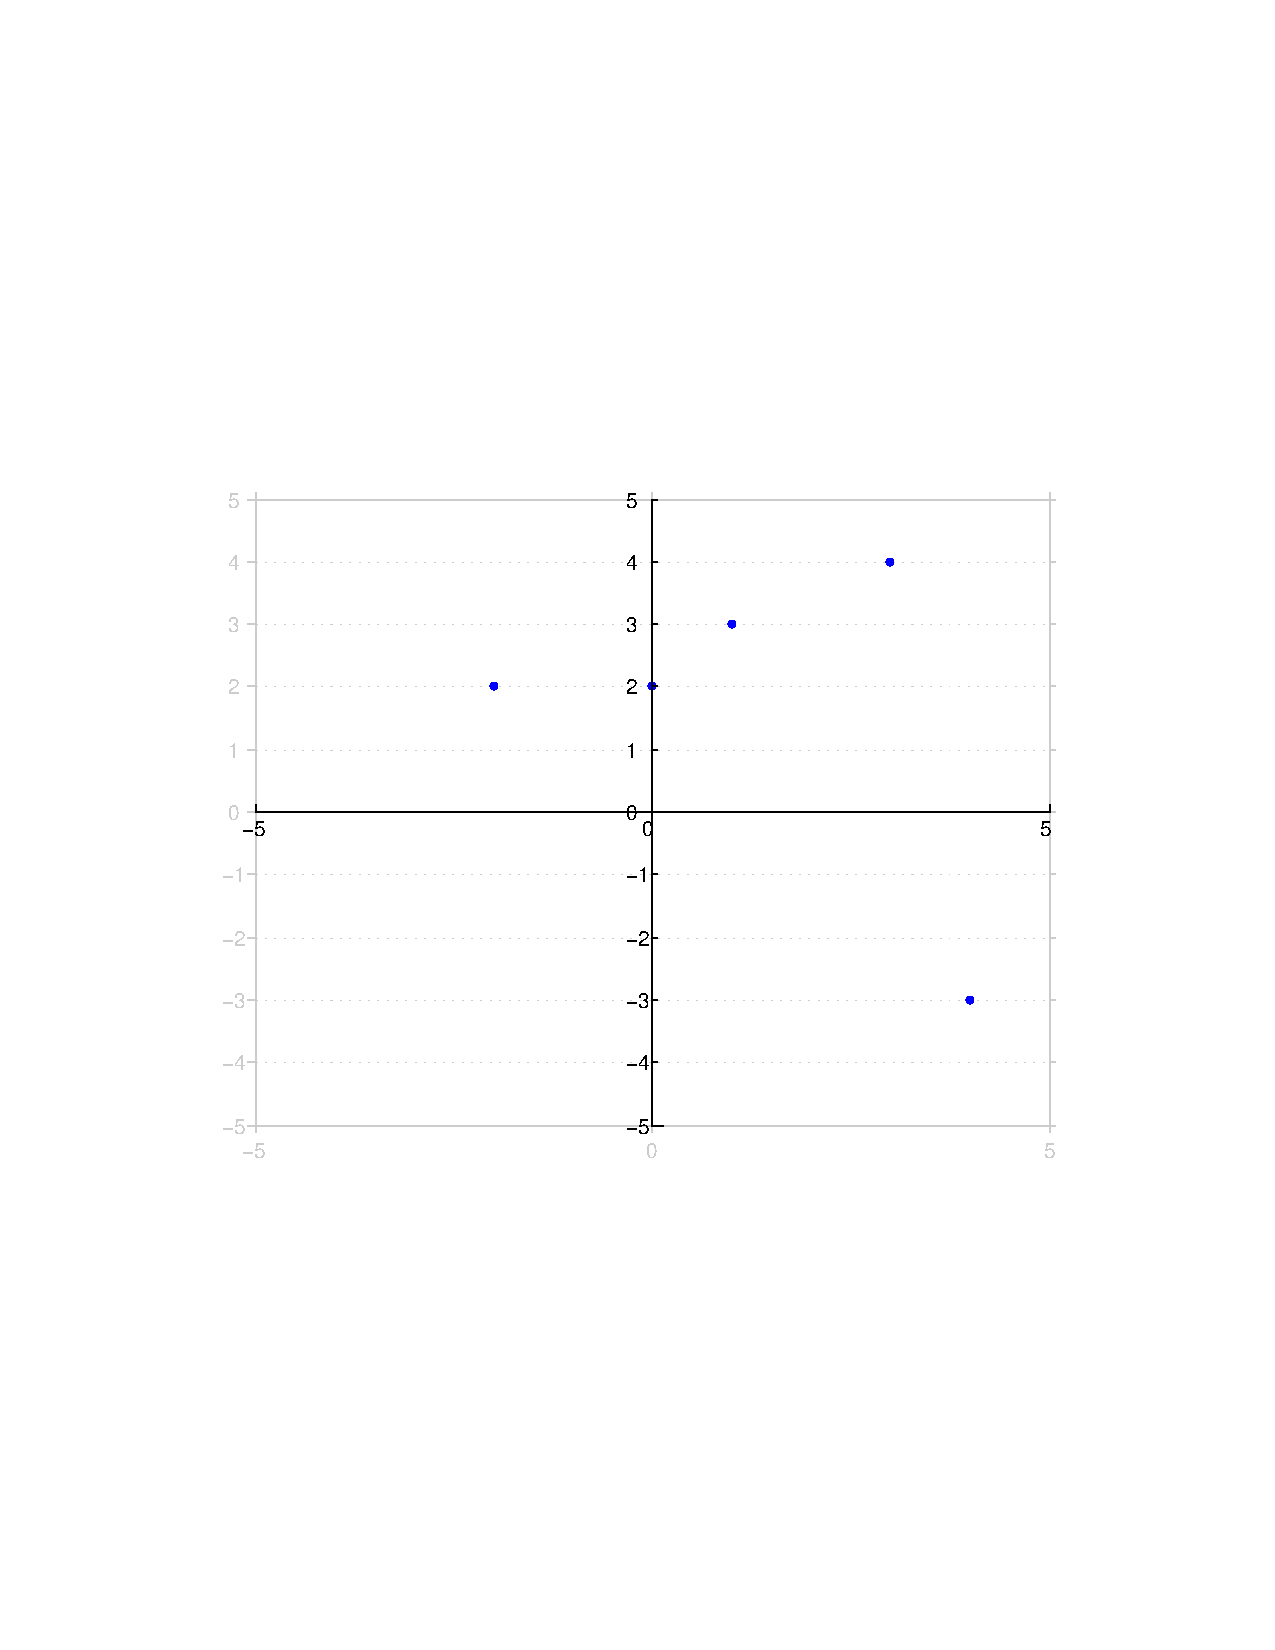
\includegraphics[width=0.5\textwidth]{matlab/es}
\end{figure}


L'intersection
\chapter{Elementary Algebra}

\section{Identities}
\begin{eqnarray}
	(a+b)^2=a^2+2ab+b^2\\
	(a-b)^2=a^2-2ab+b^2\\
	(a+b)^3=a^3+3a^2b+3ab^2+b^3\\
	(a-b)^3=a^3-3a^2b+3ab^2+b^3\\
	(a+b)^n={n\choose 0}a^n+{n\choose 1}a^{n-1}b+{n\choose 2}a^{n-2}b^2+\dots+{n\choose k}a^{n-k}b^k+\dots+{n\choose n}b^n\\
	a^2-b^2=(a-b)(a+b)\\
	a^2+b^2=(a-ib)(a+ib)\\
	a^3-b^3=(a-b)(a^2+ab+b^2)=(a-b)\left(a+(1+i\sqrt3)\frac{b}{2}\right)\left(a+(1-i\sqrt3)\frac{b}{2}\right)\\
	a^3-b^3=(a+b)(a^2-ab+b^2)=(a-b)\left(a-(1+i\sqrt3)\frac{b}{2}\right)\left(a-(1-i\sqrt3)\frac{b}{2}\right)\\
	a^n-b^n=(a-b)(a^{n-1}+a^{n-2}b+\dots+ab^{n-2}+b^{n-1}\\
	(a+b+c)^2=a^2+b^2+c^2+2ab+2bc+2ac
\end{eqnarray}

\section{Powers and roots}
$a, b>0$ and $\sqrt[n]{a}$ is only defined for $n\in\mathbb N^*$.
\begin{eqnarray}
	a^0=1\\
	a^p=a\cdot a^{p-1}\\
	a^{-q}=\frac{1}{a^q}\\
	a^{\frac{1}{q}}=\sqrt[q]{a}\\
	a^{\frac{p}{q}}=\sqrt[q]{a^p}\\
	a^pa^q=a^{p+q}\\
	\frac{a^p}{a^q}=a^{p-q}\\
	(a^p)^q=a^{p\cdot q}\\
	a^pb^p=(ab)^p\\
	\frac{a^p}{b^p}=\left(\frac{a}{b}\right)^p
	\left(\sqrt[n]{a}\right)^n=a\\
	\left(\sqrt[q]{a}\right)^p=\sqrt[q]{a^p}\\
	\sqrt[p]{\sqrt[q]{a}}=\sqrt[pq]{a}=a^{\frac{1}{pq}}\\
	\sqrt[p]{a}\sqrt[p]{b}=\sqrt[p]{ab}=(ab)^{\frac{1}{p}}\\
	\frac{\sqrt[p]{a}}{\sqrt[p]{b}}=\sqrt[p]{\frac{a}{b}}=\frac{a}{b}^{\frac{1}{p}}
\end{eqnarray}

\section{Absolute Value}
\begin{eqnarray}
	|a|=\begin{cases}
		a & a\geq0\\
		-a & a<0
	\end{cases}
\end{eqnarray}

\begin{eqnarray}
	|a|\cdot |b|=|ab|\\
	\frac{|a|}{|b|}=|\frac{a}{b}|\\
	\sqrt{a^2}=|a|\\
	\left ||a|-|b|\right |\leq |a+b|\leq |a| + |b|
\end{eqnarray}
\section{Means}
\begin{tabular}{|l|c|c|}
	\hline
	\textbf{Mean} & \textbf{of two numbers $a_1$ and $a_2$} & \textbf{of $n$ numbers $a_1, a_2,\dots$}\\
	\hline
	Arithmetic (A) & $\frac{a_1+a_2}{2}$ & $\frac{\sum_{i=1}^na_i}{n}$\\
	Weighted (W)& $\frac{\lambda_1a_1+\lambda_2a_2}{\lambda_1+\lambda_2}$ & $\frac{\sum_{i=1}^n\lambda_ia_i}{\sum_{i=1}^n\lambda_i}$\\
	Geometric (G)& $\sqrt{a_1a_2}$ & $\sqrt[n]{\prod_{i=1}^na_i}$\\
	Harmonic (H)& $\frac{2}{\frac{1}{a_1}+\frac{1}{a_23}}$ & $\frac{n}{{\sum_{i=1}^n\frac{1}{a_i}}}$\\
	Quadratic (Q)& $\sqrt{\frac{a_1^2+a_2^2}{2}}$ & $\sqrt{\frac{\sum_{i=1}^na_i^2}{n}}$\\
	\hline
\end{tabular}

Property
\begin{eqnarray}
	H\leq G\leq A\leq Q
\end{eqnarray}

\section{Polynomes}
\begin{eqnarray}
	P(x)=\sum_{k=0}^na_kx^k
\end{eqnarray}
\emph{Zeros} are $x_i$ that satisfies $P(x_i)=0$.
\subsection{Second degree polynome}
\begin{eqnarray}
	f(x)=ax^2+bx+c&a\neq0
\end{eqnarray}
Can always be rewritten
\begin{eqnarray}
	f(x)=a(x-x_0)(x-x_1)
\end{eqnarray}
where $x_0$ and $x_1$ are the \emph{zeros} of $f(x)$.
Zeros can be determined as follows
\begin{eqnarray}
	x_0,x_1=\frac{-b\pm\sqrt{\Delta}}{2a}\\
	\Delta=b^2-4ac
\end{eqnarray}

For $\Delta$ we have the following properties
\begin{eqnarray}
	\text{if }\Delta>0\text{, then }x_0,x_1\in\mathbb R\\
	\text{if }\Delta=0\text{, then }x_0=x_1\\
	\text{if }\Delta<0\text{, then }x_0,x_1\in\mathbb C
\end{eqnarray}
\begin{myExample}
	Find the zeros of $f(x)=x^2+7x+12$
	
	\begin{eqnarray*}
		\Delta = 7^2-4\cdot1\cdot12=1\\
		x_0=\frac{-7+1}{2}=-3\\
		x_1=\frac{-7-1}{2}=-4
	\end{eqnarray*}
	And $f(x)$ can be rewritten
	\begin{eqnarray*}
		f(x)=(x+4)(x+3)
	\end{eqnarray*}
\end{myExample}

\begin{myExample}
	Find the zeros of $f(x)=2x^2-5x+\frac{25}{4}$
	
	\begin{eqnarray*}
		\Delta = 5^2-4\cdot2\cdot\frac{25}{8}=-25\\
		\sqrt{\Delta}=5i\\
		x_0=\frac{5+5i}{4}=\frac{5}{4}(1+i)\\
		x_1=\frac{5-5i}{4}=\frac{5}{4}(1-i)
	\end{eqnarray*}
	Thus $f(x)$ can be rewritten
	\begin{eqnarray*}
		f(x)=2\left(x-\frac{5}{4}(1+i)\right)\left(x+\frac{5}{4}(i-1)\right)
	\end{eqnarray*}
\end{myExample}

\begin{myExample}
	Find the zeros of $f(x)=x^2+x+1$
	
	\begin{eqnarray*}
		\Delta = 1^2-4\cdot1\cdot1=-3\\
		\sqrt{\Delta}=\sqrt{3}i\\
		x_0=\frac{-1+\sqrt{3}i}{2}\\
		x_1=-\frac{1+\sqrt3i}{2}
	\end{eqnarray*}
	Thus $f(x)$ can be rewritten
	\begin{eqnarray*}
		f(x)=\left(x+\frac{1+\sqrt3i}{2}\right)\left(x+\frac{1-\sqrt{3}i}{2}\right)
	\end{eqnarray*}
\end{myExample}
La relation de Viète nous dit que pour $f(x)=ax^2+bx+c$, les zéros $x_0$ et $x_1$ satisfont
\begin{eqnarray}
	\begin{cases}
		x_0+x_1=\frac{b}{a}\\
		x_0x_1=\frac{c}{a}
	\end{cases}
\end{eqnarray}
\chapter{La droite} 
\begin{eqnarray}
	f(x)=ax+b
\end{eqnarray}

exemple de la piscine, + abo
\chapter{La parabole}
\chapter{Les fonctions polynomiales}
\chapter{Les fonctions rationelles}
%\chapter{Les fonctions transcendantes}

\chapter{Algèbre élémentaire}


\begin{tikzpicture}[
    scale=5,
    axis/.style={very thick, ->, >=stealth'},
    important line/.style={thick},
    dashed line/.style={dashed, thin},
    pile/.style={thick, ->, >=stealth', shorten <=2pt, shorten
    >=2pt},
    every node/.style={color=black}
    ]
    % axis
    \draw[axis] (-0.1,0)  -- (1.1,0) node(xline)[right]
        {$G\uparrow/T\downarrow$};
    \draw[axis] (0,-0.1) -- (0,1.1) node(yline)[above] {$E$};
    % Lines
    \draw[important line] (.15,.15) coordinate (A) -- (.85,.85)
        coordinate (B) node[right, text width=5em] {$Y^O$};
    \draw[important line] (.15,.85) coordinate (C) -- (.85,.15)
        coordinate (D) node[right, text width=5em] {$\mathit{NX}=x$};
    % Intersection of lines
    \fill[red] (intersection cs:
       first line={(A) -- (B)},
       second line={(C) -- (D)}) coordinate (E) circle (.4pt)
       node[above,] {$A$};
    % The E point is placed more or less randomly
    \fill[red]  (E) +(-.075cm,-.2cm) coordinate (out) circle (.4pt)
        node[below left] {$B$};
    % Line connecting out and ext balances
    \draw [pile] (out) -- (intersection of A--B and out--[shift={(0:1pt)}]out)
        coordinate (extbal);
    \fill[red] (extbal) circle (.4pt) node[above] {$C$};
    % line connecting  out and int balances
    \draw [pile] (out) -- (intersection of C--D and out--[shift={(0:1pt)}]out)
        coordinate (intbal);
    \fill[red] (intbal) circle (.4pt) node[above] {$D$};
    % line between out og all balanced out :)
    \draw[pile] (out) -- (E);
\end{tikzpicture}

\begin{tikzpicture}[scale=1.5]
    % Draw axes
    \draw [<->,thick] (0,2) node (yaxis) [above] {$y$}
        |- (3,0) node (xaxis) [right] {$x$};
    % Draw two intersecting lines
    \draw (0,0) coordinate (a_1) -- (2,1.8) coordinate (a_2);
    \draw (0,1.5) coordinate (b_1) -- (2.5,0) coordinate (b_2);
    % Calculate the intersection of the lines a_1 -- a_2 and b_1 -- b_2
    % and store the coordinate in c.
    \coordinate (c) at (intersection of a_1--a_2 and b_1--b_2);
    % Draw lines indicating intersection with y and x axis. Here we use
    % the perpendicular coordinate system
    \draw[dashed] (yaxis |- c) node[left] {$y'$}
        -| (xaxis -| c) node[below] {$x'$};
    % Draw a dot to indicate intersection point
    \fill[red] (c) circle (2pt);
\end{tikzpicture}
\begin{tikzpicture}[scale=2]
  \shade[top color=blue,bottom color=gray!50] 
      (0,0) parabola (1.5,2.25) |- (0,0);
  \draw (1.05cm,2pt) node[above] 
      {$\displaystyle\int_0^{3/2} \!\!x^2\mathrm{d}x$};

  \draw[style=help lines] (0,0) grid (3.9,3.9)
       [step=0.25cm]      (1,2) grid +(1,1);

  \draw[->] (-0.2,0) -- (4,0) node[right] {$x$};
  \draw[->] (0,-0.2) -- (0,4) node[above] {$f(x)$};

  \foreach \x/\xtext in {1/1, 1.5/1\frac{1}{2}, 2/2, 3/3}
    \draw[shift={(\x,0)}] (0pt,2pt) -- (0pt,-2pt) node[below] {$\xtext$};

  \foreach \y/\ytext in {1/1, 2/2, 2.25/2\frac{1}{4}, 3/3}
    \draw[shift={(0,\y)}] (2pt,0pt) -- (-2pt,0pt) node[left] {$\ytext$};

  \draw (-.5,.25) parabola bend (0,0) (2,4) node[below right] {$x^2$};
\end{tikzpicture}

\begin{tikzpicture}[scale=0.25] 
\draw [gray] (0,0) grid (13,13); 
\draw [thick] 
(0,0) -- ++(8,0) -- ++(0,3) -- cycle; 
\end{tikzpicture}

\begin{comment}
\begin{tikzpicture}[domain=0:4]
    \draw[very thin,color=gray] (-0.1,-1.1) grid (3.9,3.9);
    \draw[->] (-0.2,0) -- (4.2,0) node[right] {$x$};
    \draw[->] (0,-1.2) -- (0,4.2) node[above] {$f(x)$};
    \draw[color=red] plot[id=x] function{x} 
        node[right] {$f(x) =x$};
    \draw[color=blue] plot[id=sin] function{cos(x)} 
        node[right] {$f(x) = \sin x$};
    \draw[color=orange] plot[id=exp] function{0.05*exp(x)} 
        node[right] {$f(x) = \frac{1}{20} \mathrm e^x$};
\end{tikzpicture}
\end{comment}
\chapter{Trigonométrie}
\begin{eqnarray}
	\sin x = y \Leftrightarrow \arcsin y=x & -1\leq x\leq 1 & \frac{\pi}{2}\leq y\leq\frac{\pi}{2}\\
	\cos x = y \Leftrightarrow \arccos y=x & -1\leq x\leq 1 & 0\leq y\leq\pi\\
	\tan x = y \Leftrightarrow \arctan y=x &x\in\mathbb R&-\frac{\pi}{2}\leq y\leq \frac{\pi}{2}
\end{eqnarray}
\section{Valeurs exacts des fonctions trigonométriques d'arcs particuliers}
\begin{tabular}{| c|c|c|c|}
    \hline
	$\alpha$ & $\cos\alpha$ & $\sin\alpha$ & $\tan\alpha$\\
    \hline
    $0\textdegree$  0 & 1 & 0 & 0\\
    \hline
	$30\textdegree$ $\frac{\pi}{6}$ & $\frac{\sqrt{3}}{2}$ & $\frac{1}{2}$ & $\frac{\sqrt 3}{3}$\\
	\hline
	$45\textdegree$ $\frac{\pi}{4}$ & $\frac{\sqrt{2}}{2}$ & $\frac{\sqrt 2}{2}$ & $1$\\
	\hline
	$60\textdegree$ $\frac{\pi}{3}$  & $\frac{1}{2}$ & $\frac{\sqrt{3}}{2}$ & $\sqrt 3$\\
	\hline
	$90\textdegree$ $\frac{\pi}{2}$  & $0$ & $1$ & -\\
	\hline
 \end{tabular}
\section{Périodicité des fonctions trigonométriques}
\begin{eqnarray}
	\cos{(\alpha+2\pi)}=\cos{(\alpha)}\\
	\sin{(\alpha+2\pi)}=\sin{(\alpha)}\\
	\tan{(\alpha+\pi)}=\tan{(\alpha)}
\end{eqnarray}
\section{Relations entre fonctions trigononmétriques d'un même arc}
\begin{tabular}{|l|l|l|}
    \hline
	$\cos^2{(\alpha)}+\sin^2{(\alpha)}=1$ &
	$\tan{(\alpha)}=\frac{\sin{(\alpha)}}{\cos{(\alpha)}}$ &
	$\cot{(\alpha)}=\frac{\cos{(\alpha)}}{\sin{(\alpha)}}$ \\
	$\cot{(\alpha)}=\frac{1}{\tan{(\alpha)}}$ &
	$\frac{1}{\cos^2{(\alpha)}}=1+\tan^2{(\alpha)}$ &
	$\frac{1}{\sin^2{(\alpha)}}=1+\cot^2{(\alpha)}$  \\
	\hline
\end{tabular}
\section{Relations entre fonctions trigononmétriques de certains arcs}
\begin{tabular}{|l|l|l|}
    \hline
	$\cos{(-\alpha)}=\cos{(\alpha)}$ & $\sin{(-\alpha)}=-\sin{(\alpha)}$ & $\tan{(-\alpha)}=-\tan{(\alpha)}$ \\
   % \hline
	$\cos{(\pi-\alpha)}=-\cos{(\alpha)}$ & $\sin{(\pi-\alpha)}=\sin{(\alpha)}$ & $\tan{(\pi-\alpha)}=-\tan{(\alpha)}$ \\
    %\hline
	$\cos{(\pi+\alpha)}=-\cos{(\alpha)}$ & $\sin{(\pi+\alpha)}=-\sin{(\alpha)}$ & $\tan{(\pi+\alpha)}=\tan{(\alpha)}$ \\
    %\hline
	$\cos{\left(\frac{\pi}{2}-\alpha\right)}=\sin{(\alpha)}$ & $\sin{\left(\frac{\pi}{2}-\alpha\right)}=\cos{(\alpha)}$ &
	$\tan{\left(\frac{\pi}{2}-\alpha\right)}=\cot{(\alpha)}$ \\
    %\hline
	$\cos{\left(\frac{\pi}{2}+\alpha\right)}=-\sin{(\alpha)}$ & $\sin{\left(\frac{\pi}{2}+\alpha\right)}=\cos{(\alpha)}$ &
	$\tan{\left(\frac{\pi}{2}+\alpha\right)}=-\cot{(\alpha)}$ \\
    \hline

 \end{tabular}
\\\\
\underline{Remarques:} ces relations peuvent être facilement retrouvées en utilisant la formule de Moivre: $e^{j\phi}=\cos{\phi}+j\sin{\phi}$, voir le chapitre sur les nombres complexes.
\section{Conversion des mesures d'angles}
On note respectivement $d,r, m$ et $g$ la mesure d'angle en degrés, en radians, en minutes et en grades.

Pour un même angle, on a 
\begin{eqnarray}
	\frac{d}{180}=\frac{r}{\pi}=\frac{m}{30}=\frac{g}{200}
\end{eqnarray}
\part{Analysis in $\mathbb{R}$}
%!TEX root = /Users/Johan/Documents/University/Math/Gymnase/book/book.tex
\chapter{Dérivée}
\section{Fonction composée}
\begin{myDefinition}
	$y=f(u)$ $u=g(x)$ $y=f(g(x))=(f\circ g)(x)$
\end{myDefinition}
\begin{myExample}
	
	
	$y=f(u)=\sqrt{u}$ 
	\\
	$u=g(x)=x^2+1$
	\\
	$y=(f\circ g)(x)$
	Calculer $f'(x)$.
	
	\begin{eqnarray*}
		f'(u)=\frac{1}{2}u^{-\frac{1}{2}}
		\\
		g'(x)=2x
		\\
		(f\circ g)'(x)=f'(g(x))g'(x)=\frac{x}{\sqrt{x^2+1}}
	\end{eqnarray*}
\end{myExample}
\begin{eqnarray}
	f'(x)=\frac{dy}{dx}(x)=\lim_{\Delta x\rightarrow 0}\frac{f(x+\Delta x)-f(x)}{\Delta x}
\end{eqnarray}
\begin{eqnarray}
	\frac{d}{dx}(af(x))=a\frac{d}{dx}f(x)
	\\
	\frac{d}{dx}\left(f(x)+g(x)\right)=	\frac{d}{dx}f(x)+\frac{d}{dx}g(x)
	\\
	\frac{d}{dx}\left((f\circ g)(x)\right)=(f \circ g)' = (f'\circ g) \cdot g'
	\\
	(f\cdot g)'=f'\cdot g+f\cdot g'
	\\
	\frac{f}{g}=\frac{f'\cdot g-f\cdot g'}{g^2}
\end{eqnarray}

\textbf{Exemple:}

\begin{eqnarray*}
	\left(7\frac{x^2+x+5}{e^{2x}}\right)'
\end{eqnarray*}
On peut récrire sous la forme suivante
\begin{eqnarray}
	\left(a\frac{f}{g}\right)'=a\left(\frac{f}{g}\right)'=a\frac{f'\cdot g-f\cdot g'}{g^2}
\end{eqnarray}
où $a=7$, $f=x^2+x+5$ et $g=e^{2x}$. 

On a $f'(x)=2x+1$ et $g'(x)=2e^{2x}$ et obtient donc:
\begin{eqnarray*}
	\left(7\frac{x^2+x+5}{e^{2x}}\right)'=7\frac{e^{2x}((2x+1)-2\cdot(x^2+x+5))}{4e^{4x}}
	=-\frac{7}{4}\frac{2x^2+9}{e^{2x}}
\end{eqnarray*}

Pour $y=f(x)\Rightarrow dy=f'(x)\Delta x=f'(x)dx$, on a $dx=\Delta x$ \underline{\textbf{mais}} $dy\neq\Delta y$!

\begin{eqnarray}
	\Delta y=f(x+\Delta x)-f(x)\text{ ou }	\Delta y+f(x)=f(x+\Delta x)
\end{eqnarray}

\begin{myExample}
	$y=3x^2-5$, $x=2$ et $\Delta x=0.1$
	Calculer $\Delta y$ et $dy$.
	
	Tout d'abord on remarque que $\Delta x=dx$ et $f'(x)=6x$.
	\begin{eqnarray*}
		\Delta y=f(x+\Delta x)-f(x)=f(2.1)-f(2)=1.23
	\end{eqnarray*}
	et
	\begin{eqnarray*}
		dy=\frac{dy}{dx}dx=f'(x)dx=f'(x)\Delta x=f'(2)\cdot0.1=1.2
	\end{eqnarray*}
	
\end{myExample}

\section{Dérivée de fonctions implicites}
si $y^4+3y-4x^3=5x+1$ défini sur une fonction implicite $f(x)$, alors on dérive tous les termes par $x$ et on factorise par $y'$.
\begin{eqnarray*}
	(y^4)'+(3y)'-(4x^3)'=(5x)'+(1)'=
	\\
	4y^3y'+3y'-12x^2=5
	\\
	y'(4y^3+3)=12x^2+5
\end{eqnarray*}
et
\begin{eqnarray*}
	y'=f'(x)=\frac{12x^2+5}{4(f(x))^3+3}
\end{eqnarray*}
\begin{myExample}
	Taux liés
	
	Soit $x^3-2y^2+5x=16$, $\frac{dx}{dt}=4$, $x=2$, $y=-1$ et $\frac{dy}{dt}=?$
	\begin{eqnarray*}
		\frac{d}{dt}(x^3)'-\frac{d}{dt}(2y^2)'+\frac{d}{dt}(5x)'=\frac{d}{dt}(16)
		\\
		3x^2\frac{dx}{dt}-4y\frac{dy}{dt}+5\frac{dx}{dt}=0
		\\
		3\cdot2^2\cdot4-4\cdot(-1)\frac{dy}{dt}+5\cdot 4=0
		\\
		\Rightarrow \frac{dy}{dt}=\frac{-20-48}{4}=-17
	\end{eqnarray*}
\end{myExample}
\chapter{Applications de la dérivée}
\section{Extremums}
Si $f(x)$ est continue et que $f'(x)=0$ a une solution cette dernière est un point critique (max, min, point de selle).

\begin{myExample}
	\begin{eqnarray*}
		f(x)=2\sin{(x)}+\cos{(2x)}
		\\
		f'(x)=2\cos{(x)}-2\sin{(2x)}=2\cos{(x)}-4\sin{(x)}\cos{(x)}=2\cos{(x)}(1-2\sin{(x)})
	\end{eqnarray*}
	Il nous faut donc trouver les solutions du système d'équation suivant
	\begin{eqnarray*}
		\begin{cases}
			\cos{(x)}=0
			\\
			1-2\sin{(x)}=0 \Leftrightarrow \frac{1}{2}=\sin{(x)}
		\end{cases}	
	\end{eqnarray*}
	La solution de la première équation est $x=(1+2k)\pi$, la résolution de la deuxième équation est un peu plus délicate mais on trouve
	\begin{eqnarray*}
		x=\begin{cases}
			\frac{\pi}{6}+2k\pi
			\\
			-\frac{\pi}{6}+(1+2k)\pi
		\end{cases}
	\end{eqnarray*}
	Les extremums de $f(x)$ sont donc donnés par
	\begin{eqnarray*}
		x=\begin{cases}
			(1+2k)\pi
			\\
			\frac{\pi}{6}+2k\pi
			\\
			-\frac{\pi}{6}+(1+2k)\pi
		\end{cases}
	\end{eqnarray*}
	avec $k\in\mathbb Z$.
\end{myExample} 

\section{Théorème des accroissements finis}
Si $f$ est une fonction continue sur l'intervalle fermé $[a,b]$ est dérivable sur l'intervalle ouvert $]a,b[$, tel que $a<b$ et $f(a)=f(b)$. $f'(c)=0$, avec $c\in]a,b[$, en au moins un point de $]a,b[$.

\begin{myTheorem}\textbf{Théorème de accroissements finis}
	Si $f$ est dérivable sur $[a,b]$ alors \begin{eqnarray}
		f'(c)=\frac{f(b)-f(a)}{b-a}
	\end{eqnarray} 
\end{myTheorem}

\section{Test de la dérivée première}
Soit $f$ continue sur $[a,b]$ et dérivable sur $]a,b[$
\begin{enumerate}
	\item si $f'(x)>0$  fonction croissante
	\item si $f'(x)<0$  fonction décroissante
	\item si $f'(x)=0$  point critique
\end{enumerate}
\section{Concavité et test de la dérivée seconde}
	\begin{enumerate}
		\item si f''(x)>0 convexe
		\item si f''(x)<0 non convexe (concave)
		\item si f''(x)=0 point d'inflexion (Wendepunkt)
	\end{enumerate}
\section{Problème d'optimisation}
\begin{enumerate}
	\item créer une fonction représentant la donnée du problème
	\item dériver
	\item déterminer quelle genre d'optimum on trouve et quel genre d'optimum on cherche. Attention aux "rand"max qui sont déterminés par la donnée du problème et qui ne correspondent pas forcément à l'optimum trouvé.
\end{enumerate}

\begin{myExample}
	$f(x)=(32-2x)x$, $f'(x)=32-4x$, $\hat x=8$
\end{myExample}

\section{Méthode de Newton}	
La méthode de Newton est une méthode numérique permettant de trouver les zéros d'une fonction, pour plus de détails se référer au cours d'analyse numérique.

Soit $f(x)$ une fonction continue sur $[a,b]$, une approximation de $f(x)=0$ peut être donnée par
\begin{eqnarray}
	x^{(k+1)}=x^{(k)}-\frac{f(x^{(k)})}{f'(x^{(k)})}
\end{eqnarray}
où $x^{(0)}\in[a,b]$ est choisi arbitrairement.

\begin{myExample}
On cherche les zéros de	$f(x)=x-\cos{(x)}$.

On a $f'(x)=1-\sin{(x)}$ la méthode s'écrit donc
\begin{eqnarray*}
	x^{(k+1)}=x^{(k)}-\frac{x^{(k)}-\cos{(x^{(k)})}}{1-\sin{(x^{(k)})}}
\end{eqnarray*}
en prenant $x^{(0)}=0.8$ on a
\begin{eqnarray*}
	x^{(0)}=& &0.8
	\\
	x^{(1)}=&0.8-\frac{0.8-\cos{(0.8)}}{1-\sin{(0.8)}}=&0.74
	\\
	x^{(2)}=&\cdots&0.739
	\\
	x^{(3)}=&\cdots&0.739
	\\
	x^{(4)}=&\cdots&0.739085133\dots
\end{eqnarray*}
\end{myExample}

\section{The differential operator: ${\rm d}$}
The $\rm d$ operator indicates an infinitely small interval.

\begin{equation}
	\lim_{\Delta x\rightarrow0}\Delta x={\rm d}x
\end{equation}
\section{Operator Algebra}
The operator $\rm d$ followed by its associated variable can be treated as a common variable and allows to find interesting and practical identities. Be aware that the operator is not dissociable from its attached variable; not allowed to divide by ${\rm d}$! For instance
\begin{eqnarray}
	\frac{{\rm d} x^2}{{\rm d}x}=2x\\
	\Rightarrow
	{\rm d}x^2 =2x{\rm d}x
\end{eqnarray}

or

\begin{eqnarray}
	\frac{{\rm d} \ln{(x)}}{{\rm d}x}=\frac{1}{x}\\
	\Rightarrow
	{\rm d} \ln{(x)} =\frac{1}{x}{\rm d}x
\end{eqnarray}

The latter proves that a percentage change can simply be expressed as the derivative of the $\log$ function.
\begin{equation}
	\frac{\dot x}{x} = \frac{{\rm d} \ln{(x)}}{{\rm d}t}
\end{equation}
In discrete time, we find the following approximation for small changes
\begin{equation}
	\frac{x_1-x_0}{x_0}\approx\ln{\left(\frac{x_1}{x_0}\right)}
\end{equation}

More generally, one can state
\begin{equation}
	{\rm d}f(x) = \left(\frac{{\rm d}f(x)}{{\rm d}x}\right){\rm d}x=f'(x){\rm d}x
\end{equation}


\begin{myExample}
	In physics it is know that work is the line integral of the force:
	\begin{equation}
		W_\Gamma = \int_{\Gamma} Fd\gamma.
	\end{equation}
	
	So the instantaneous force can be retrieved by differentiating $W$ at $\mathbf{x}$.
	
	When the $W$ is only potential energy, i.e. $W=U=mgh = mg(x-0)$ it is very easy to retrieve the gravity force.
	
	\begin{equation}
		F = \frac{{\rm d} U}{{\rm d} x} = mg.
	\end{equation}
	
	
	Now, if we do the same exercie with work that comprises only kinetic energy, i.e. $W=K=\frac{1}{2}mv^2$, one can retrieve Newton's second law by using operator algebra.
	
	\begin{enumerate}
		\item Rewrite $v$ in the differental form
		\begin{equation}
			K = \frac{1}{2}m\left(\frac{{\rm d}x}{{\rm d} t}\right)^2
		\end{equation}
		
		\item apply differentiation rigorously and methodically, also to operators
		\begin{eqnarray}
			\frac{\rm d K}{{\rm d}x} 
			&=& \frac{\rm d}{{\rm d}x}\left(\frac{1}{2}m\left(\frac{{\rm d}x}{{\rm d}t}\right)^2\right)\\
			&=& \frac{1}{2}m\frac{\rm d}{{\rm d}x}\left(\left(\frac{{\rm d}x}{{\rm d}t}\right)^2\right)\\
			&=& \frac{m}{2{\rm d}t^2}\frac{\rm d}{{\rm d}x}\left(\left({\rm d}x\right)^2\right)\\
			&=& \frac{m}{2{\rm d}t^2}\frac{2{\rm d}x}{{\rm d}x}{\rm d}{\rm d}x\\
			&=& m \frac{{\rm d}^2x}{{\rm d}t^2}\\
			&=& ma
		\end{eqnarray}
	\end{enumerate}
\end{myExample}


 
\chapter{Intégrales}
\section{Primitives et intégrales définies}
$F(x)$ est primitive de $f(x)$, si $F'(x)=f(x)$
\begin{eqnarray}
	\int f(x)dx=F(x)+C
\end{eqnarray}
\section{Changement de variables dans les intégrales définies}
si $F$ est primitive de $f$
\begin{eqnarray}
	\int f(g(x))g'(x)dx=F(g(x))+C
\end{eqnarray}
si $u=g(x)$ et $du=g'(x)dx$
\begin{eqnarray}
	\int f(u)du=F(u)+C
\end{eqnarray}

\begin{myExample}

	\begin{eqnarray*}
		\int\sqrt{5x+7}dx & u=5x+7 & du=5dx
		\\
		\int\sqrt u\frac{1}{5}du=\frac{1}{5}\frac{2}{3}u^{\frac{3}{2}}+C=\frac{2}{15}(5x+7)^{\frac{3}{2}}+C
	\end{eqnarray*}
	
\end{myExample}

\section{Symbole de sommation et aires}
\underline{Notation:} $\sum_{k=0}^{n}=a_0+a_1+a_2+\dots+a_n$

On peut approximer une intégrale en utilisant des rectangles sous la courbe.
\begin{eqnarray*}
	A=(x_1-x_0)f(x_0)+(x_2-x_1)f(x_1)+\dots+(x_n-x_{n-1})f(x_{n-1})
	\\
	A=\sum_{k=0}^{n}\Delta xf(x_k)=\Delta x\sum_{k=0}^nf(x_k)
\end{eqnarray*}

\section{Intégrale définie}
\begin{eqnarray}
	A=\int_a^bf(x)dx=F(b)-F(a)
\end{eqnarray}

\section{Théorème fondamental du calcul intégral}
\begin{eqnarray}
	\int_a^bf(x)dx=F(b)-F(a)
\end{eqnarray}
\begin{itemize}
	\item si $f$ impaire ($f(-x)=-f(x)$):
	\begin{eqnarray}
		\int_{-a}^a f(x)dx=0
	\end{eqnarray}
	\item si $f$ paire ($f(x)=f(-x)$):
	\begin{eqnarray}
	\int_{-a}^af(x)dx=2\int_0^af(x)dx
	\end{eqnarray}
\end{itemize}
	
\section{Intégration numérique}

Pour plus de détails sur les intégrations numériques, se référer au cours d'analyse numérique.
\subsection{Méthode des trapèzes}
\begin{eqnarray}
	\int_a^bf(x)dx=\left(\frac{b-a}{n}\sum_{k=0}^nf(x_k)\right)-f(x_0)-f(x_n)
\end{eqnarray}
\subsection{Méthode de Simpson}
\begin{eqnarray}
	\int_a^bf(x)dx
	=\frac{b-a}{3n}\left[f(x_0)+4f(x_1)+2f(x_2)+4f(x_3)+\dots+f(x_{n-2})+4f(x_{n-1})+f(x_n)\right]
\end{eqnarray}
avec $n$ pair.

\chapter{Applications de l'intégrale définie}

\section{Aires}
\begin{eqnarray}
	A=\int_a^b\left(g(x)-f(x)\right)dx
\end{eqnarray}

\section{Solides de révolution}
\begin{eqnarray}
	V=\pi\int_a^b(f(x)^2)dx
\end{eqnarray}

\section{Valeurs par les tubes cylindriques}
\begin{eqnarray}
	V=2\pi\int_a^bxf(x)dx
\end{eqnarray}
\begin{myExample}
	Calculer le volume sous la paraboloïde: $f(x)=x^2+c$ avec $c>0$ délimitée par le disque $x^2+y^2=r^2$.
	\\\\
	On pose
	\begin{eqnarray*}
		V=2\pi\int_0^{r}xf(x)dx=
		\\
		2\pi\int_0^{r}x^3+cxdx=
		\\
		2\pi\left[\frac{x^4}{4}+c\frac{x^2}{2}\right]_0^r=
		\\
		\pi r^2\left[\frac{r^2}{2}+c\right]
	\end{eqnarray*}
	
\end{myExample}

\section{Valeurs d'après les sections transversales}
\begin{eqnarray}
	V=\int_a^bA(x)dx
\end{eqnarray}

\begin{myExample}
	On veut calculer le volume d'une pyramide de base $a \times a$ et de hauteur $h$.
	\\\\
	%mettre schéma indispensable ici pour une bonne compréhension
	On a\begin{eqnarray*}
		A(x)=(2y)^2=4y^2
	\end{eqnarray*}
	En suivant un raisonnement géométrique, on a
	\begin{eqnarray*}
		\frac{y}{x}=\frac{\frac{1}{2}a}{h}
		\\
		\Rightarrow
		y=\frac{ax}{2h}
	\end{eqnarray*}
	On peut donc écrire
	\begin{eqnarray*}
		A(x)=\frac{a^2x^2}{h^2}
	\end{eqnarray*}
	et donc
	\begin{eqnarray*}
		V=\int_0^h\frac{a^2x^2}{h^2}dx
		\\
		=\frac{a^2}{h^2}\int_0^hx^2dx
		\\
		=\frac{a^2}{h^2}\left[\frac{x^3}{3}\right]_0^h
		\\
		V=\frac{a^2}{3}h
	\end{eqnarray*}
\end{myExample}

\section{Longueur d'arc et surface de révolution}
\begin{eqnarray}
	L_a^b=\int_a^b\sqrt{1+(f'(x))^2}dx
\end{eqnarray}
\subsection{Abscisse curviligne}
\begin{eqnarray}
	s(x)=\int_a^x\sqrt{1+(f'(t))^2}dt
\end{eqnarray}
et
\begin{eqnarray}
	ds=\sqrt{1+(f'(x))^2}dx
\end{eqnarray}
$\rightarrow$ approximation de la longueur.

\section{Surface de révolution}
\begin{eqnarray}
	S=\int_a^b2\pi f(x)\sqrt{1+(f'(x))^2}dx
\end{eqnarray}
%!TEX root = /Users/Johan/Documents/University/Math/Gymnase/book.tex
\chapter{Fonctions logarithmiques et exponentielles}
\section{Fonctions réciproques}

\begin{myDefinition}
	\textbf{Injective} $f(x)$ et injective quand $f(a)\neq f(b)\Leftrightarrow a\neq b$, c-à-d la fonction n'a jamais deux fois la même valeur, elle est donc soit strictement croissante ou décroissante.
\end{myDefinition}

\begin{myDefinition}
	\textbf{Réciproque} $y=f(x) \Leftrightarrow x=g(y)$, alors $g(y)$ est la fonction réciproque de $f(x)$.

On note la réciproque de $f$, $f^{-1}(x)$.

On a également la propriété suivante: $f(f^{-1}(x))=f^{-1}(f(x))=x$

Si $g(x)=f^{-1}(x)$ alors $g'(x)=\frac{1}{f'(g(x))}$
\end{myDefinition}

\begin{myExample}
	$f(x)=3x-5$, trouver la fonction réciproque.\\\\
	On pose tout d'abord $y=f(x)$ et donc $y=3x-5$. Par raisonnement algébrique on trouve $x=\frac{y+5}{3}$ et donc $f^{-1}(x)=\frac{x+5}{3}$
\end{myExample}
\section{Logarithme naturel}
\begin{myDefinition}
	\begin{eqnarray}
		\ln{x}=\int_1^x\frac{1}{t}dt
	\end{eqnarray}
	On en déduit tout de suite que
	\begin{eqnarray}
		\frac{d}{dx}\ln{x}=\frac{1}{x}
	\end{eqnarray}
\end{myDefinition}

On a les propriétés suivantes:
\begin{eqnarray}
	\ln{(ab)}=ln{a}+\ln{b}
	\\
	\ln{\frac{a}{b}}=\ln{a}-\ln{b}
	\\
	\ln{a^b}=b\ln{a}
\end{eqnarray}
\subsection{Dérivation logarithmique}
\begin{eqnarray*}
	y=f(x)
	\\
	\ln y=\ln f(x)
	\\
	\frac{1}{y}y'=\frac{f'(x)}{f(x)}=(\ln{f(x)})'
\end{eqnarray*}
\begin{myExample}
	\begin{eqnarray*}
		y=\frac{(5x-4)^3}{\sqrt{2x-1}}
		\\
		\ln{y}=\ln{\left(\frac{(5x-4)^3}{\sqrt{2x-1}}\right)}
		\\
		=\ln{\left((5x-4)^3\right)}-\ln{\left(\sqrt{2x-1}\right)}
		\\
		=3\ln{(5x-4)}-\frac{1}{2}\ln{(2x-1)}
	\end{eqnarray*}
	Maintenant il est facile d'obtenir une dérivée.
	\begin{eqnarray*}
		(\ln{y})'=3\frac{5}{5x-4}-\frac{1}{2}\frac{2}{2x-1}=\frac{15}{5x-4}-\frac{1}{2x-1}
	\end{eqnarray*}
\end{myExample}
\section{Fonction exponentielle}
\begin{myDefinition}
	La fonction exponentielle est la fonction réciproque du logarithme.
	\begin{eqnarray}
		e^x=\exp{x}=y \Leftrightarrow x=\ln y
	\end{eqnarray}
	On a donc 
	\begin{eqnarray}
		\exp{(\ln{y})}=\ln{(e^y)}=y
	\end{eqnarray}
	Notons que $e^1=e\backsimeq 2.71828\dots$
\end{myDefinition}
On a les relations sivantes
\begin{eqnarray}
	e^pe^q=e^{p+q}
	\\(e^{p})^r=e^{pr}
	\\
	\label{eq:expdiff}(e^x)'=e^x
	\\
	(e^u)^r=u'e^u
	\end{eqnarray}
Notez l'équation \ref{eq:expdiff} qui est particulièrement intéressante. L'exponentielle est la seule fonction à posséder cette propriété; $f(x)=f'(x)$.
\section{intégration}
\begin{eqnarray}
	\int\frac{1}{u}du=\ln |u|+C
	\\
	\int e^udu=\frac{e^u}{u'}+C
	\\
	\int\tan{(u)}du=-\ln{|\cos{u}|}+C
	\\
	\int\cot{u}du=\ln{|\cos{u}|}+C
	\\
	\int\sec{u}du=\ln{|\sec{u}+\tan{u}|}+C
	\\
	\int\csc{u}du=\ln{|\csc{u}+\cot{u}|}+C
\end{eqnarray}
\textbf{Rappel:}
\begin{eqnarray}
	\tan^{-1}{u}=\cot{u}
	\\
	\sin^{-1}{u}=\csc{u}
	\\
	\cos^{-1}{u}=\sec{u}
\end{eqnarray}

\section{Fonctions exponentielles et logarithmes de bases quelconque}
\begin{eqnarray}
	a^x=e^{x\ln{(a)}}
	\\
	(a^x)'=a^x\ln{a}
	\\
	(a^u)'=a^u\ln{(a)}u'
	\\
	\int a^xdx=\frac{a^x}{\ln{(a)}}
	\\
	\int a^udx=\frac{a^u}{\ln{(a)}u'}
\end{eqnarray}

\begin{eqnarray}
	y=\log_ax\Leftrightarrow x=a^y
	\\
	\log_ax=\frac{\ln x}{\ln a}
\end{eqnarray}

\begin{eqnarray}
	(\log_ax)'=\left(\frac{ln x}{\ln a}\right)'=\frac{1}{\ln(a)}\frac{1}{x}
\end{eqnarray}

Pour prouver que $\log_ax=\frac{\ln{x}}{\ln{a}}$, on part de
\begin{eqnarray*}
	a^y=x
\end{eqnarray*}
Par définition, on a
\begin{eqnarray*}
	\log_a{a^y}=y=\log_a x
\end{eqnarray*}
Mais aussi
\begin{eqnarray*}
	\ln{a^y}=y\ln{a}=\ln{x}
\end{eqnarray*}
et donc
\begin{eqnarray*}
	y=\frac{\ln{x}}{\ln{a}}=\log_ax
\end{eqnarray*}
Notons que ce résultat se généralise aisément pour obtenir
\begin{eqnarray}
	\log_a{x}=\frac{\log_bx}{\log_ba}
\end{eqnarray}
On peut vérfier le théorème précédent de la façon suivante
\begin{eqnarray*}
	\ln{(x)}=\log_a{(x)}\ln{(a)}=\ln{(a^{\log_a{(x)}})}\\
	x=a^{\log_a{(x)}}=x
\end{eqnarray*}

\section{Loi de croissance}
\begin{eqnarray}
	y(t)=y_0e^{kt}
\end{eqnarray}
où $y_0$ est la valeur initiale, à $t=0$. $y_0$ a la même unité que $y$.
$k$ est une constante d'unité $[\frac{1}{s}]$, si elle est multipliée au temps $t$. L'exposant, ici $kt$, n'a jamais d'unité.

\section{Factorial}
\begin{equation}
	n! = \prod_{k=1}^n k  = n\cdot(n-1)\cdot(n-2)...\cdot1
\end{equation}
where $k\in\mathbb N$

\subsection{Stirling's Approximation}
for large values of $n$, $n!$ can be approximated as following
\begin{equation}
	n! \approx \sqrt{2\pi n}\left(\frac{n}{e}\right)^n.
\end{equation}

\subsection{Binomial Coefficients}
\begin{equation}
	\binom nk = \frac{n!}{(n-k)!k!}
\end{equation}

\chapter{Fonctions trigonométriques réciproques et hyperboliques}
\section{Dérivées et intégrales}
\begin{eqnarray}
	\frac{d}{dx}\arcsin u = \frac{1}{\sqrt{1-u^2}}\frac{du}{dx}\\
	\frac{d}{dx}\arccos u = -\frac{1}{\sqrt{1-u^2}}\frac{du}{dx}\\
	\frac{d}{dx}\arctan u = \frac{1}{\sqrt{1+u^2}}\frac{du}{dx}
%	\frac{d}{dx}\arcsc u = \frac{1}{u\sqrt{u^2-1}}\frac{du}{dx}\\
\end{eqnarray}

\begin{eqnarray}
	\int\frac{1}{\sqrt{a^2-u^2}}du=\arcsin{\left(\frac{u}{a}\right)}+C\\
	\int\frac{1}{\sqrt{a^2+u^2}}du=\frac{1}{a}\arctan{\left(\frac{u}{a}\right)}+C
	%\int\frac{1}{u\sqrt{u^2-a^2}}du=\frac{1}{a}\arcsec{\left(\frac{u}{a}\right)}+C\\
\end{eqnarray}

\section{Fonctions hyperboliques}
\begin{eqnarray}
	\cosh{(x)}=\frac{e^x+e^{-x}}{2}\\
	\sinh{(x)}=\frac{e^x-e^{-x}}{2}
\end{eqnarray}

\subsection{Propriétés}
\begin{eqnarray}
	\cosh^2{(x)}-\sinh^2{(x)}=1
\end{eqnarray}
\subsection{Dérivées et intégrales}
\begin{eqnarray}
	\frac{d}{dx}\sinh{(x)}=\cosh{(x)}\frac{du}{dx}\\
	\frac{d}{dx}\cosh{(x)}=\sinh{(x)}\frac{du}{dx}
\end{eqnarray}

\section{Fonctions hyperboliques réciproques}
% todo checker si c'est arg ou Arg et qu'est que la différence ...
\begin{eqnarray}
	\arg\sinh{(x)}=\ln{(x+\sqrt{x^2+1})}\\
	\arg\cosh{(x)}=\ln{(x+\sqrt{x^2-1})}
\end{eqnarray}
$\arg$ est l'argument.
\subsection{Dérivées et intégrales}
\begin{eqnarray}
	\frac{d}{dx}\arg\sinh{(x)}=\frac{1}{\sqrt{u^2+1}}\frac{du}{dx}\\
	\frac{d}{dx}\arg\cosh{(x)}=\frac{1}{\sqrt{u^2-1}}\frac{du}{dx}
\end{eqnarray}

\begin{eqnarray}
	\int\frac{1}{\sqrt{u^2+a^2}}du=\arg\sinh{\left(\frac{u}{a}\right)}+C\\
	\int\frac{1}{\sqrt{u^2-a^2}}du=\arg\cosh{\left(\frac{u}{a}\right)}+C
\end{eqnarray}
%!TEX root = /Users/Johan/Documents/University/Math/Gymnase/book/book.tex
\chapter{Techniques d'intégration}
\section{Intégration par parties}
\begin{myDefinition}
	\begin{eqnarray}
		\int f(x)g'(x)dx=f(x)g(x)-\int f'(x)g(x)dx
	\end{eqnarray}
	$\int udv=uv-\int vdu$
\end{myDefinition}
\begin{myExample}
	\begin{eqnarray*}
		\int xe^{2x}dx=?
	\end{eqnarray*}
	\\
	$dv=e^{2x}dx$, $v=\frac{1}{2}e^{2x}$, $u=x$ et $du=dx$
	\begin{eqnarray*}
		\int xe^{2x}dx=
		\\
		\int u\frac{dv}{dx}dx=uv-\int\frac{du}{dx}vdx=
		\\
		x\frac{1}{2}e^{2x}-\int \frac{1}{2}e^{2x}dx=
		\\e^{2x}\left(\frac{x}{2}-\frac{1}{4}\right)+C
	\end{eqnarray*}
\end{myExample}
\begin{myExample}
	\begin{eqnarray*}
		\int\ln{(x)}dx=?
	\end{eqnarray*}
	\\
	On pose $dv=dx$, $v=x$, $du=\frac{1}{x}$ et $u=\ln{(x)}$
	\begin{eqnarray*}
		\int\ln{(x)}\cdot 1dx=x\ln{(x)}-\int1\cdot dx=x(\ln{(x)}-1)
	\end{eqnarray*}
\end{myExample}
\section{Substitutions}
a faire
%todo
\section{Intégrales trigonométriques}
Pour une intégrale du type
\begin{eqnarray*}
	\int\sin^n{(x)}dx
\end{eqnarray*}
utiliser $\sin^2{(x)}=1-\cos^2{(x)}$.
\begin{myExample}
	\begin{eqnarray*}
		\int\sin^5{(x)}dx=\int\sin^4{(x)}\sin{(x)}dx=\int\left(1-\cos^2{(x)}\right)^2\sin{(x)}dx
		\\
		\int\left(1-2\cos^2{(x)}+\cos^4{(x)}\right)\sin{(x)}dx
	\end{eqnarray*}
	On pose $u=\cos{(x)}$ et $du=-\sin{(x)}$ et notre expression devient
	\begin{eqnarray*}
		\int\sin^5{(x)}dx=-\int\left(1-2u^2+u^4\right)du=-u+\frac{2}{3}u^3-\frac{1}{5}u^5+C
	\end{eqnarray*}
On peut utiliser le même principe pour une puissance impaire de $\cos{(x)}$, on remplace simplement par $1-\sin{(x)}$ cette fois.
\end{myExample}

Pour une puissance paire de $\cos$ ou $\sin$ utiliser les substitutions suivantes: $\sin^2{(x)}=\frac{1}{2}(1-\cos{(2x)})$ et $\cos^2{(x)}=\frac{1}{2}(1+\cos{(2x)})$.
\begin{myExample}
	\begin{eqnarray*}
		\int\sin^4{(x)}dx=\frac{1}{4}\int(1-\cos{(2x)})^2dx=\frac{1}{4}\int1-2\cos{(2x)}+\cos^2{(2x)}dx
	\end{eqnarray*}
	on remplace $\cos^2{(2x)}=\frac{1+\cos{(4x)}}{2}$ ce qui donne
	\begin{eqnarray*}
		\int\sin^4{(x)}dx=\frac{1}{4}\int1-2\cos{(2x)}+\frac{1+\cos{(4x)}}{2}dx=\frac{3}{8}x-\frac{1}{4}\sin{(2x)}+\frac{1}{32}\sin{(4x)}+C
	\end{eqnarray*}
\end{myExample}

\section{Substitutions trigonométriques}
%todo be done
\section{Intégrales de fonctions rationelles}

\begin{myExample}
	Le but est d'intégrer
	\begin{eqnarray*}
		\int\frac{4x^2+13x-9}{x^3+2x^2-3x}dx
	\end{eqnarray*}
	La clé dans ce genre de problème est de faire une décomposition en éléments simples. Tout d'abord on remarque que
	\begin{eqnarray*}
		x^3+2x^2-3x=x(x^2+2x-3)=x(x-1)(x+3).
	\end{eqnarray*}
	On pose
	\begin{eqnarray*}
		\frac{4x^2+13x-9}{x^3+2x^2-3x}=\frac{A}{x}+\frac{B}{x-1}+\frac{C}{x+3}
		\\
		\Rightarrow 4x^2+13x-9=A(x-1)(x+3)+Bx(x+3)+Cx(x-1)
	\end{eqnarray*}
	Quand $x=0$: $-3A=-0\Rightarrow A=3$\\
	quand $x=1$: $4B=8\Rightarrow B=2$\\
	et quand $x=-3$: $12C=-12\Rightarrow C=-1$.
	
	On a donc
	\begin{eqnarray*}
		\frac{4x^2+13x-9}{x^3+2x^2-3x}=\frac{3}{x}+\frac{2}{x-1}-\frac{1}{x+3}
	\end{eqnarray*}
	et
	\begin{eqnarray*}
		\int\frac{4x^2+13x-9}{x^3+2x^2-3x}dx=\int\frac{3}{x}+\frac{2}{x-1}-\frac{1}{x+3}dx
		\\
		=\int\frac{3}{x}dx+\int\frac{2}{x-1}dx-\int\frac{1}{x+3}dx\\
		=3\ln{|x|}+2\ln{|x-1|}-\ln{|x+3|}+C\\
		=\ln{\left|\frac{x^3(x-1)^2}{x+3}\right|}+C
	\end{eqnarray*}
\end{myExample}

\section{Intégrales d'expressions quadratiques}
Si $ax^2+bx+c$ est irréductible on peut effectuer la marche à suivre illustrée dans l'exemple suivant.
\begin{myExample}
	On veut calculer
	\begin{eqnarray*}
		\int\frac{2x-1}{x^2-6x+13}dx
	\end{eqnarray*}
	On remarque que $\Delta=36-4\cdot13=-16<0$, on récrit donc l'expression
	\begin{eqnarray*}
		x^2-6x+13=x^2-6x+9+13-9=(x-3)^2+4
	\end{eqnarray*}
	On pose $u=x-3$ et $du=dx$, et on obtient
	\begin{eqnarray*}
		\int\frac{2x-1}{x^2-6x+13}dx=\int\frac{2x-1}{(x-3)^2+4}dx=\int\frac{2u+5}{u^2+4}du
		\\=2\int\frac{u}{u^2+4}du+5\int\frac{1}{u^2+4}du=\ln{\left|u^2+4\right|}+\frac{5}{2}\arctan{\left|\frac{u}{2}\right|}+C
		\\
		=\ln{\left|x^2-6x+13\right|}+\frac{5}{2}\arctan{\left|\frac{x-3}{2}\right|}+C
	\end{eqnarray*}
\end{myExample}

\chapter{Les formes indéterminées $\frac{0}{0}$ et $\frac{\infty}{\infty}$}
\section{La règle de l'Hôpital}
\begin{myTheorem}
	Si\begin{eqnarray*}
		\lim_{x \to c}f(x)=\lim_{x \to c}g(x)=0\text{ ou }\infty 
	\end{eqnarray*}
	et si $\lim_{x\to c}f'(x)/g'(x)$ existe, alors
	\begin{eqnarray}
		\lim_{x\to c}\frac{f(x)}{g(x)} = \lim_{x\to c}\frac{f'(x)}{g'(x)}.
	\end{eqnarray}
\end{myTheorem}

\begin{myExample}
	On veut calculer
	\begin{eqnarray*}
		\lim_{x\rightarrow0}\frac{\cos{(x)}+2x-1}{3x}
	\end{eqnarray*}
	On remarque qu'on tombe sur une forme indéterminée ($\frac{0}{0}$). En dérivant l'expression du haut et du bas on trouve
	\begin{eqnarray}
		\lim_{x\rightarrow0}\frac{\cos{(x)}+2x-1}{3x}=\lim_{x\rightarrow0}\frac{\sin{(x)}+2}{3}=\frac{2}{3}
	\end{eqnarray}
\end{myExample}
\chapter{Suites}
Une \textbf{suite} est une application de $\mathbb N$ (ou d'une partie de $\mathbb N$) vers $\mathbb R$. L'image de $n\in\mathbb N$ par cette application, notée $u_n$, converge vers un nombre réel $a$ si $\lim_{n\rightarrow+\infty}u_n=a$.

\begin{enumerate}
	\item Une suite croissante et majorée converge
	\item Une suite décroissante et minorée converge
\end{enumerate}

\section{Suite arithmétique}
La suite $u_1,u_2,u_3,\dots$ est une suite \textbf{arithmétique} de raison $r$ si, pour tout $n\in\mathbb N^*, u_{n+1}=u_n+r$.

\begin{eqnarray}
	u_n=u_1+(n-1)r\\
	\sum_{i=1}^{n}u_i=n\frac{u_1+u_n}{2}
\end{eqnarray}

\section{Suite géométrique}
La suite $u_1,u_2,u_3,\dots$ est une suite \textbf{géométrique} de raison $r$ si, pour tout $n\in\mathbb N^*, u_{n+1}=r\cdot u_n$.
\begin{eqnarray}
	u_n=u_1\cdot r^{n-1}\\
	a \sum_{i=0}^{n} q^{i} =a \frac{1-q^{n+1}}{1-q}\\
	\lim_{n\rightarrow+\infty}\sum_{i=0}^{n} q^{i}=\frac{1}{1-q}&|q|<1
\end{eqnarray}

\subsection{Proof}
One very elegant proof is to consider the following equation
\begin{equation*}
	\label{eq:beginprooffseriegeom}
	x = 1+ax
\end{equation*}
we know $x= \frac{1}{1-a}$

We substitute $1+ax$ to $x$ on the RHS of the equation which gives
\begin{eqnarray*}
	x &=& 1+ax\\
	&=& 1 + a(1+ax)\\
	&=& 1 + a(1+a(1+x))\\
	&=& 1 + a + a^2 + a^3 + ... +a^n + a^{n+1}x\\
	&=& \sum_{k=0}^n a^k + a^{n+1}x
\end{eqnarray*}
which leads to
\begin{eqnarray*}
	\sum_{k=0}^n a^k &=&   x-a^{n+1}x= x\left(1-a^{n+1}\right)
\end{eqnarray*}
since we know from eq \ref{eq:beginprooffseriegeom} $x=\frac{1}{1-a}$, we subsitute and find
\begin{equation*}
	\sum_{k=0}^n a^k =  \left(1-a^{n+1}\right)\frac{1}{1-a}
\end{equation*}
which is the geometric serie.

\chapter{Series}
La série de termes $u_k$ convege si la suite $s_n=\sum_{k=1}^nu_k$ converge. La limite de cette suite, notée $\sum_{k=1}^\infty u_k$, est la somme de la série.
\section{Series convergentes et divergentes}
\subsection{Power serie}
Power series are defined as follows:
\begin{eqnarray}
	\sum_{n=0}^{\infty}a_nx^n
\end{eqnarray}

Two very important properties applies to those series
\begin{eqnarray}
	\sum_{n=0}^{\infty}\frac{d}{dx}a_nx^n=\frac{d}{dx}\sum_{n=0}^{\infty}a_nx^n
\end{eqnarray}
and
\begin{eqnarray}
	\sum_{n=0}^{\infty}\int_0^{x}a_nx^ndx=\int_0^x\left(\sum_{n=0}^{\infty}a_nx^n\right)dx
\end{eqnarray}

Here is one example
\begin{eqnarray*}
	\sum_{n=0}^{\infty}\frac{z^{-n}}{n}=\sum_{n=0}^{\infty}\int_0^z-z^{-n-1}dz=\int_0^z\underbrace{\left(\sum_{n=0}^{\infty}-z^{-n-1}\right)}_{-\frac{1}{1-z}}dz=-\int_0^z\frac{1}{1-z}dz=1-\ln{(1-z)}
\end{eqnarray*}


\subsection{Série géométrique}
\subsubsection{Somme de nombre consécutifs}
\begin{eqnarray}
	\sum_{i=0}^{n}i=\sum_{i=1}^ni=\frac{1}{2}n(n+1)
\end{eqnarray}
\subsubsection{Somme de carrés}
\begin{eqnarray}
	\sum_{i=0}^{n}i^2=\sum_{i=1}^ni^2=\frac{1}{3}n^3+\frac{1}{2}n^2+\frac{1}{6}n=\frac{1}{3}n\left(n+1\right)\left(n+\frac{1}{2}\right)
\end{eqnarray}
\begin{eqnarray}
	\sum_{i=0}^{n}i^3=\sum_{i=1}^ni^3=\frac{1}{4}n^2\left(n+1\right)^2
\end{eqnarray}
\begin{eqnarray}
	\sum_{i=0}^{n}i^4=\sum_{i=1}^ni^4=\frac{1}{4}n^2\left(n+1\right)^2
\end{eqnarray}
\subsection{Série téléscopique}
\section{Séries à termes positifs}
\subsection{Série de Riemann}
\section{Les tests d'Alembert et les racines}
\subsection{Critèredu quotient (Alembert)}
Si $\lim_{k\rightarrow+\infty}\frac{u_{k+1}}{u_k}=c$ et $c \begin{cases}
	c<1 \text{ , la série converge}\\c>1 \text{ , la série diverge}
\end{cases}$

\subsection{Critère de la racine (Cauchy)}
Si $\lim_{k\rightarrow+\infty}\sqrt{u_k}=\lim_{k\rightarrow+\infty}u_k^{1/k}=c$ et $\begin{cases}
	c<1\text{, la série converge}\\
	c>1\text{, la série diverge}
\end{cases}$
\section{Séries alternées et convergence absolue}
\section{Fonctions représentées par une série entière}
\section{La série du binôme}
\section{Série entière}
Une série de terme général $u_k$ est appelée \textbf{série entière} si $u_k=a_kx^k$ avec $a_k\in\mathbb R$.

Rayon de convergence: 
\begin{eqnarray}
	r=\lim_{k\rightarrow+\infty}\left|\frac{a_k}{a_k+1}\right|\\
	r=\frac{1}{\lim_{k\rightarrow+\infty}|a_k|^{1/k}}
\end{eqnarray}
La série entière de terme $a_x^k \begin{cases}
	\text{converge si }|x|<r\\
	\text{diverge si }|x|>r
\end{cases}$
Si $|x|=r$, il y a un doute.

Si $r=+\infty$, alors la série entière converge pour tout réel $x$.
\section{Exemples de séries}
\subsection{Exemples de séries divergentes}
\begin{eqnarray}
	1+\frac{1}{2}+\frac{1}{3}+\frac{1}{4}+\frac{1}{5}+\dots=\sum_{i=1}^\infty\frac{1}{i}=+\infty&\text{Série harmonique}\\
	1+\frac{1}{\sqrt 2}+\frac{1}{\sqrt 3}+\frac{1}{\sqrt 4}+\frac{1}{\sqrt 5}+\dots=\sum_{i=1}^\infty\frac{1}{\sqrt i}=+\infty
\end{eqnarray}
et plus généralement
\begin{eqnarray}
	1+\frac{1}{2^\alpha}+\frac{1}{3^\alpha}+\frac{1}{4^\alpha}+\frac{1}{5^\alpha}+\dots=\sum_{i=1}^\infty\frac{1}{i^\alpha}=+\infty&\text{si $\alpha\leq1$}
\end{eqnarray}
\begin{eqnarray}
	1+r+r^2+r^3+\dots+r^k+\dots=+\infty&\text{si $r\geq1$}
\end{eqnarray}
\subsection{Exemples de séries convergentes}
\begin{eqnarray}
	1+\frac{1}{1!}+\frac{1}{2!}+\frac{1}{3!}+\dots+\frac{1}{k!}+\dots=\sum_{k=0}^\infty\frac{1}{k!}=e\\
	1+\frac{1}{2}+\frac{1}{4}+\frac{1}{8}+\dots=\sum_{k=0}^\infty\frac{1}{2^k}=2\\
	1+r+r^2+r^3+\dots=\sum_{i=1}^{n}r^i=\frac{1}{1-r}&|r|<1
\end{eqnarray}
\begin{eqnarray}
	1+\frac{1}{2^\alpha}+\frac{1}{3^\alpha}+\dots=\sum_{k=0}^\infty\frac{1}{k^\alpha}=\zeta(\alpha)&\text{ fonction zêta de Riemann}\\
	1+\frac{1}{4}+\frac{1}{9}+\frac{1}{25}+\dots=\zeta(2)=\frac{\pi^2}{6}\\
	1+\frac{1}{16}+\frac{1}{81}+\frac{1}{256}+\dots=\zeta(4)=\frac{\pi^4}{90}\\
	1+\frac{1}{9}+\frac{1}{25}\frac{1}{49}+\dots=\sum_{k=0}^\infty\frac{1}{(2k+1)^2}=\frac{\pi^2}{8}\\
	1+\frac{1}{81}+\frac{1}{625}\frac{1}{2401}+\dots=\sum_{k=0}^\infty\frac{1}{(2k+1)^4}=\frac{\pi^4}{96}
\end{eqnarray}

\begin{eqnarray}
	\frac{1}{1\cdot2}+\frac{1}{2\cdot3}+\frac{1}{3\cdot4}+\dots=\sum_{k=1}^\infty\frac{1}{k\cdot(k+1)}=1\\
	\frac{1}{1\cdot3}+\frac{1}{3\cdot5}+\frac{1}{5\cdot7}+\dots=\sum_{k=1}^\infty\frac{1}{(2k-1)\cdot(2k+1)}=\frac{1}{2}\\
	\frac{1}{1\cdot3}+\frac{1}{2\cdot4}+\frac{1}{3\cdot5}+\dots=\sum_{k=2}^\infty\frac{1}{(k-1)\cdot(k+1)}=\frac{3}{4}\\
	\frac{1}{3\cdot5}+\frac{1}{7\cdot9}+\frac{1}{11\cdot13}+\dots=\sum_{k=1}^\infty\frac{1}{(4k-1)\cdot(4k+1)}=\frac{1}{2}-\frac{\pi}{8}
\end{eqnarray}
\begin{eqnarray}
	1-\frac{1}{1!}+\frac{1}{2!}-\frac{1}{3!}+\dots=\sum_{k=0}^\infty(-1)^k\frac{1}{k!}=\frac{1}{e}\\
	1-\frac{1}{2}+\frac{1}{3}-\frac{1}{4}+\dots=\sum_{k=0}^\infty(-1)^k\frac{1}{k+1}=\ln{2}&\text{Série harmonique alternée}\\
	1-\frac{1}{3}+\frac{1}{5}-\frac{1}{7}+\dots=\sum_{k=0}^\infty(-1)^k\frac{1}{2k+1}=\frac{\pi}{4}\\
	1-\frac{1}{4}+\frac{1}{9}-\frac{1}{16}+\dots=\sum_{k=0}^\infty(-1)^k\frac{1}{(k+1)^2}=\frac{\pi}{4}
\end{eqnarray}

\section{Formule de Taylor d'ordre $n$}
On note $f$ une fonction $n+1$ fois continuement dérivable dans un intervalle ouvert $I$ contenant $a$.

Pour tout $x\in I$:

\begin{eqnarray}
	f(x)=f(a)+\frac{1}{1!}f'(a)(x-a)+\frac{1}{2!}f''(a)(x-a)^2+\dots+\frac{1}{n!}f^{(n)}(a)(x-a)^n+R_n(x)
\end{eqnarray}
avec \begin{eqnarray}
	R_n(x)=\int_a^x\frac{1}{n!}f^{(n+1)}(t)(x-t)^ndt=\frac{1}{(n+1)!}f^{(n+1)}(c)(x-a)^{n+1}
\end{eqnarray} où $c$ est compris entre $a$ et $x$.

Estimation du reste: $|R_n(x)|\leq\frac{|x-a|^{n+1}}{(n+1)!}\mathrm{sup}_{t\in I}{|f^{(n+1)}(t)|}$.

Si $\lim_{n\rightarrow+\infty}R_n(x)=0$, alors $f(x)=\sum_{k=0}^\infty\frac{1}{k!}f^{(k)}(a)(x-a)^k$ et la série de terme $\frac{1}{k!}f^{(k)}(a)(x-a)^k$ est appelée \textbf{série de Taylor de $f$ contrée en $a$}.
\subsection{Formule de MacLaurin}
Si $a=0$, on obient la formule de MacLaurin:
\begin{eqnarray}
	f(x)=f(0)+\frac{1}{1!}f'(0)x+\frac{1}{2!}f''(0)x^2+\dots+\frac{1}{n!}f^{(n)}(0)x^n+R_n(x)
\end{eqnarray}
\chapter{Sujets de géométrie analytique}
\section{Parabole}
\section{Ellipse}
\section{Hyperbole}
\subsection{Rotation d'axe}
\part{Analysis in $\mathbb{R}^n$}
\chapter{Courbes planes et coordonnées polaires}
\section{Courbes planes}
\section{Tangentes et longueur d'arc}
\section{Coordonnées polaires}
\section{Intégrales en coordonnées polaires}
\section{Equation polaire des coniques}
\chapter{Vecteurs et surfaces}
\section{Produit scalaire}
\section{Produit vectoriel}
\section{Droites et plans}

\chapter{Fonctions vectorielles}
\chapter{Dérivation partielle}
\section{fonction de plusieurs variables}
\begin{equation}
	f(x, y, z)
\end{equation}
ou plus généralement
\begin{equation}
	f ( \mathbf{x})
\end{equation}
\section{Limites et continiuité}
même chose que pour une variable: la variable d'intérêt varie et les autres restent fixées.
\section{Dérivée partielle}
\begin{equation}
	\frac{\partial f}{\partial x} = \lim_{\Delta x\rightarrow 0} \frac{f(x+\Delta x, y, z)-f(x, y, z)}{\Delta x}
\end{equation}
\subsection{Exemple}
For $f(x,y,z)=x^2+3y+\sin{(z)}$, 
\begin{eqnarray}
	\label{eq:deriveepartielle}
	\frac{\partial f}{\partial x} &=& 2x\nonumber\\
	\frac{\partial f}{\partial y} &=& 3\nonumber\\
	\frac{\partial f}{\partial z} &=& \cos{(z)}
\end{eqnarray}

\section{Dérivée de fonctions composées}
\section{Dérivée directionelle}
\section{Normales et plans tangents}
\section{Valeurs extrêmes des fonctions à plusieurs variables}

\section{Gradient}
\begin{equation}
	\nabla = \begin{pmatrix}
		\frac{\partial}{\partial x_1}\\
		\vdots\\
		\frac{\partial}{\partial x_n}
	\end{pmatrix}
\end{equation}

Hence the example eq \ref{eq:deriveepartielle} can be rewritten
\begin{equation}
	\nabla f =
	\begin{pmatrix}
		2x \\ 3 \\ \cos{(z)}
	\end{pmatrix}
\end{equation}



\section{Total derivative}
\begin{equation}
	{\rm d} f = 
	\frac{\partial f}{\partial t}{\rm d}t +
	\frac{\partial f}{\partial x}{\rm d}x +
	\frac{\partial f}{\partial y}{\rm d}y +
	\frac{\partial f}{\partial z}{\rm d}z
\end{equation}

More generally

\begin{equation}
	{\rm d}f=\sum\limits_{i=1}^n \frac{\partial f}{\partial x_i}\, {\rm d}x_i\,\,.
\end{equation}

In vector form, this writes

\begin{eqnarray}
	{\rm d}f&=&
	\begin{pmatrix}
		\frac{\partial f}{\partial t}&
		\frac{\partial f}{\partial x}&
		\frac{\partial f}{\partial y}&
		\frac{\partial f}{\partial z}
	\end{pmatrix}
	\cdot
	\begin{pmatrix}
		{\rm d}t\\{\rm d}x\\{\rm d}y\\{\rm d}z
	\end{pmatrix}\\
	&=&\nabla f\cdot {\rm d}\mathbf{x}
\end{eqnarray}

\subsection{Application: error calculation}

\begin{equation}
	\Delta f \approx
	\frac{\partial f}{\partial t}\Delta t +
	\frac{\partial f}{\partial x}\Delta x +
	\frac{\partial f}{\partial y}\Delta y +
	\frac{\partial f}{\partial z}\Delta z
\end{equation}
works for small $\Delta$.
\part{Linear Algebra}
\chapter{Grands concepts}
\begin{myDefinition}
	Matrices $m\times n$ où $m$ est le nombre de lignes et $n$ le nombre de colonnes.
\end{myDefinition}
\begin{eqnarray*}
	\begin{cases}
		4x_1+6x_2+9x_3=6\\
		6x_1+2x_3=20\\
		5x_1-8x_2+x_3=10
	\end{cases}
\end{eqnarray*}
Le système ci-dessus peut être récrit sous la forme suivante
\begin{eqnarray*}
	\begin{bmatrix}
		4 &6& 9\\
		6  &0 &-2\\
		5 & -8 & 1
	\end{bmatrix}
	\begin{bmatrix}
		x_1\\x_2\\x_3
	\end{bmatrix}
	=\begin{bmatrix}
		6\\20\\10
	\end{bmatrix}
	%\mathbf{Ax}=\mathbf{B}
\end{eqnarray*}


\section{Matrix addition and scalar multiplication}
\begin{myDefinition}
	Sum of two matrices $A[a_{jk}]$ and $B[b_{jk}]$ of the same size.
	\begin{eqnarray}
		\textbf{A+B}=
		\begin{bmatrix}
			a_{11}+b_{11} & a_{12}+b_{12} & \cdots & a_{1n}+b_{1n}
			\\
			\vdots & & & \vdots
			\\
			a_{m1}+b_{m1} & a_{m2}+b_{m2} & \cdots & a_{mn}+b_{mn}
		\end{bmatrix}
	\end{eqnarray}
\end{myDefinition}
\section{Multiplying by a scalar}
\begin{myDefinition}
	\begin{eqnarray}
		c\textbf{A}=
		\begin{bmatrix}
			ca_{11}&ca_{12}&\cdots&ca_{1n}
			\\
			\vdots&&&\vdots
			\\
			ca_{m1}&ca_{m2}&\cdots&ca_{mn}
		\end{bmatrix}	
	\end{eqnarray}
	
\end{myDefinition}
\section{Matrix multiplication}
\begin{eqnarray}
	\mathbf{A}\cdot \mathbf{B}=\mathbf{C} 
\end{eqnarray}

\begin{eqnarray}
	\mathbf{A}\cdot \mathbf{B}\neq\mathbf{B}\cdot \mathbf{A}
\end{eqnarray}
[n x m][m x p]=[n x p]
\begin{eqnarray}
	c_{jk}=\sum_{i=1}^na_{ji}b_{ik}
\end{eqnarray}
\begin{myExample}
	Exemple de multiplication d'une matrice $2\times2$ par une matrice $2\times1$.
	\begin{eqnarray*}
		\begin{pmatrix}
			4 & 2 \\ 1 & 8
		\end{pmatrix}
		\cdot
		\begin{pmatrix}
			3\\5
		\end{pmatrix}
		=
		\begin{pmatrix}
			4\cdot3+2\cdot5 \\ 1\cdot3+8\cdot5
		\end{pmatrix}
		=\begin{pmatrix}
			22\\43
		\end{pmatrix}.
	\end{eqnarray*}
	Exemple de multiplication d'une matrice $2\times3$ par une matrice $3\times3$.
	\begin{eqnarray*}
		\begin{pmatrix}
			1 & 2 & 3
			\\
			4 & 5 & 6
		\end{pmatrix}
		\cdot
		\begin{pmatrix}
			3 & 2 & 0
			\\
			1 & 0 & 6
			\\
			1 & 1 & 0
		\end{pmatrix}
		=\begin{pmatrix}
			1\cdot3+2\cdot1+3\cdot1 & 1\cdot2+2\cdot0+3\cdot1 & 1\cdot0+2\cdot6+3\cdot0
			\\
			4\cdot3+5\cdot1+6\cdot1 & 4\cdot2+5\cdot0+6\cdot1 & 4\cdot0+5\cdot6+6\cdot0
		\end{pmatrix}
		=\begin{pmatrix}
			8 & 5 & 12
			\\
			23 & 14 & 30
		\end{pmatrix}
	\end{eqnarray*}
\end{myExample}

\section{Transposition}
\begin{myDefinition}
	si $\mathbf{A}[a_{jk}]$, alors $\mathbf{A^T}[a_{kj}]$.
	\begin{eqnarray}
		\mathbf{A^T}=[a_{kj}]=
		\begin{pmatrix}
			a_{11} & a_{21} & \cdots & a_{n1}
			\\
			\vdots & & &\vdots
			\\
			a_{1m} & a_{2m} &\cdots & a_{nm}
		\end{pmatrix}
	\end{eqnarray}
\end{myDefinition}
\begin{myExample}
	\begin{eqnarray*}
		\mathbf{A}=
		\begin{pmatrix}
			5 & -8 & 1
			\\
			4 & 0 & 7
		\end{pmatrix}
	\end{eqnarray*}
	Alors
	\begin{eqnarray*}
		\mathbf{A^T}=
		\begin{pmatrix}
			5 & 4\\
			-8&0\\
			1& 7
		\end{pmatrix}
	\end{eqnarray*}
\end{myExample}

\subsection{Propriétés}
\begin{eqnarray}
	\mathbf{(A^T)^T}=\mathbf{A}
	\\
	\mathbf{A^T}+\mathbf{B^T}=\mathbf{(A+B)^T}\\
	\mathbf{A^TB^T}=\mathbf{(AB)^T}
\end{eqnarray}

\begin{myDefinition}
	Symmetric matrix
	\begin{eqnarray}
		\mathbf{A}=\mathbf{A^T}
	\end{eqnarray}
	Skew symmetric matrix
	\begin{eqnarray}
		\mathbf{A^T}=-\mathbf{A}
	\end{eqnarray}
	thus $a_{jk}=-a_{kj}$ and $a_{jj}=0$.
\end{myDefinition}

\begin{myDefinition}
	Triangular matrix
	\begin{itemize}
		\item upper triangular
		\begin{eqnarray}
			a_{jk}=0&j>k
		\end{eqnarray}
		\underline{Example}
		\begin{eqnarray*}
			\begin{pmatrix}
				1 & 4 & 3\\
				0 & 5 & -8\\
				0 & 0 & 7
			\end{pmatrix}
		\end{eqnarray*}
		\item lower triangular
		\begin{eqnarray}
			a_{jk}=0&j<k
		\end{eqnarray}
		\underline{Example}
		\begin{eqnarray*}
			\begin{pmatrix}
				2 & 0 & 0\\
				8&-1&0\\
				7&6&8
			\end{pmatrix}
		\end{eqnarray*}
	\end{itemize}
\end{myDefinition}

\section{Identity Matrix}
\begin{myDefinition}
	\begin{eqnarray}
		a_{jj}=1&a_{jk}=0&\forall j\neq k
	\end{eqnarray}
	\begin{eqnarray}
		\mathbf{I}=
		\begin{pmatrix}
			1 & 0 & 0 & \cdots & 0\\
			0 & 1 & 0 & \cdots & 0\\
			0 & 0 & 1 & \cdots & 0\\
			\vdots &  &  & \cdots & \vdots\\
			0 & 0 & 0 &\cdots & 1
			
		\end{pmatrix}
	\end{eqnarray}
\end{myDefinition}
\begin{myDefinition}
	Diagonal Matrix
	\begin{eqnarray}
		\mathbf{A}=c\mathbf{I}
	\end{eqnarray}
\end{myDefinition}

\section{Linear Systems of Equations}
\subsection{Gauss Elimination}
\begin{myExample}
	\begin{eqnarray*}
		\begin{cases}
			x_1-x_2+x_3=0\\
			-x_1+x_2-x_3=0\\
			10x_2+25x_3=90\\
			20x_1+10x_2=80
		\end{cases}
		\\
		\Rightarrow
		\\
		\begin{pmatrix}
			1 & -1 & 1 & 0\\
			-1&1&-1&0\\
			0&10&25&90\\
			20&10&0&80
		\end{pmatrix}
	\end{eqnarray*}
	$l_1=l_2$, $\frac{l_3}{5}$ and $\frac{l4}{4}$.
	\begin{eqnarray*}
		\begin{pmatrix}
			1 & -1 & 1 & 0\\
			0&2&5&18\\
			2&1&0&8
		\end{pmatrix}
	\end{eqnarray*}
	$l_3-2l_1$
	\begin{eqnarray*}
		\begin{pmatrix}
			1 & -1 & 1 & 0\\
			0&2&5&18\\
			0&3&-2&8
		\end{pmatrix}
	\end{eqnarray*}
	$l_3-\frac{3}{2}l_2$
	\begin{eqnarray*}
		\begin{pmatrix}
			1 & -1 & 1 & 0\\
			0&2&5&18\\
			0&0&-\frac{19}{2}&-19
		\end{pmatrix}
	\end{eqnarray*}
	$-\frac{2}{19}l_3$
	\begin{eqnarray*}
		\begin{pmatrix}
			1 & -1 & 1 & 0\\
			0&2&5&18\\
			0&0&1&2
		\end{pmatrix}
	\end{eqnarray*}
	$l_2-5l_3$
	\begin{eqnarray*}
		\begin{pmatrix}
			1 & -1 & 1 & 0\\
			0&2&0&8\\
			0&0&1&2
		\end{pmatrix}
	\end{eqnarray*}
	$\frac{l_2}{2}$
	\begin{eqnarray*}
		\begin{pmatrix}
			1 & -1 & 1 & 0\\
			0&1&0&4\\
			0&0&1&2
		\end{pmatrix}
	\end{eqnarray*}
	$l_1+l_2-l_3$
	\begin{eqnarray*}
		\begin{pmatrix}
			1 & 0 & 0 & 2\\
			0&1&0&4\\
			0&0&1&2
		\end{pmatrix}
	\end{eqnarray*}
	Si on ré-écrit désormais le système, on obtient
	\begin{eqnarray*}
		\begin{cases}
			1\cdot x_1+0\cdot x_2+0\cdot x_3=2\\
			0\cdot x_1+1\cdot x_2+0\cdot x_3=4\\
			0\cdot x_2+0\cdot x_2+1\cdot x_3=2
		\end{cases}
	\end{eqnarray*}
	ce qui est équivalent à
	\begin{eqnarray*}
		\begin{cases}
			x_1=2\\
			x_2=4\\
			x_3=2
		\end{cases}
	\end{eqnarray*}
\begin{comment}
	\begin{eqnarray*}
		-\frac{19}{2}x_3=-19\Rightarrow x_3=2
		\\
		a
	\end{eqnarray*}
	

\end{comment}
\end{myExample}
\chapter{Linear Independance. Rank of a Matrix. Vector Space}
\begin{eqnarray}
	\label{eq:syslin}c_1\overrightarrow{a_1}+c_2\overrightarrow{a_2}+\dots+c_n\overrightarrow{a_n}=0
\end{eqnarray}
Si la seule solution du système \ref{eq:syslin} est $c_i=0$ pour $i=1,\dots,n$, alors les vecteurs $\overrightarrow a_i$ sont linéairement indépendants.

Le rang est le nombre de vecteurs indépendants d'une matrice.

Espace vectoriel $\mathbb R^n$ consiste de tous les vecteurs à $n$ composantes à la dimension $n$.

\section{Déterminants. Cramer's Rule}
\begin{eqnarray}
	\mathbf{D}=\det \mathbf{A}=\left|
	\begin{matrix}
		a_{11} & a_{12} & \cdots & a_{1n}
		\\
		\vdots & & & \vdots
		\\
		a_{n1} & a_{n2} & \cdots & a_{nn}
	\end{matrix}\right|
\end{eqnarray}
\begin{itemize}
	\item if $n=1$
	\begin{eqnarray}
		\det \mathbf{A}=a_{11}
	\end{eqnarray}
	\item if $n=2$
	\begin{eqnarray}
		\det \mathbf{A}=a_{11}a_{22}-a_{12}a_{21}
	\end{eqnarray}
	\item if $n=3$
	\begin{eqnarray}
		\det \mathbf{A}=a_{11}a_{22}a_{33}+a_{12}a_{23}a_{31}+a_{13}a_{21}a_{32}-a_{32}a_{23}a_{11}-a_{33}a_{21}a_{12}-a_{31}a_{22}a_{13}
	\end{eqnarray}
\end{itemize}

\begin{myDefinition}
	Matrice des signes
	\begin{eqnarray}
		\begin{pmatrix}
			+ & - & + & - & \cdots \\
			 - & + & - & + &  \cdots \\
			+ & - & + & - & \cdots \\
			 - & + & - & + & \cdots \\
			\vdots & & & \cdots
		\end{pmatrix}
	\end{eqnarray}
	This can also be expressed in the following manner
	\begin{eqnarray}
		a_{jk}=
		\begin{cases}
			+ & \text{if }(j+k)\text{ is even}
			\\
			- & \text{if }(j+k)\text{ is odd}
		\end{cases}
	\end{eqnarray}
\end{myDefinition}

\begin{myExample}
	Calculate
	\begin{eqnarray}
		\mathbf{D}=\det\mathbf{A}=
		\left|
		\begin{matrix}
			1 & 3 & 0\\
			2 & 6 & 4\\
			-1 & 0 &2
		\end{matrix}
		\right|
	\end{eqnarray}
	Using minors and cofactors one can write
	\begin{eqnarray*}
		\left|
		\begin{matrix}
			1 & 3 & 0\\
			2 & 6 & 4\\
			-1 & 0 &2
		\end{matrix}
		\right|
		=
		1
		\left|
		\begin{matrix}
			
			 6 & 4\\
			 0 &2
		\end{matrix}
		\right|
		-3
		\left|
		\begin{matrix}
		
			2  & 4\\
			-1  &2
		\end{matrix}
		\right|
		+0
		\left|
		\begin{matrix}
			
			2 & 6\\
			-1 & 0 
		\end{matrix}
		\right|
		=
		1\cdot12-3\cdot8+0=-12
	\end{eqnarray*}
\end{myExample}
\section{Evaluation of $\det$ by Reduction to Triangular Form}
\begin{myExample}
	\begin{eqnarray*}
		\mathbf{D}=\det \mathbf{A}=
		\left|
		\begin{matrix}
			2&0&-4&6\\
			4&5&1&0\\
			0&2&6&-1\\
			-3&8&9&1
		\end{matrix}
		\right|
	\end{eqnarray*}
	$l_2-2l_1$ and $l_4+\frac{3}{2}l_1$
	\begin{eqnarray*}
		\left|
		\begin{matrix}
			2&0&-4&6\\
			0&5&9&-12\\
			0&2&6&-1\\
			0&8&3&10
		\end{matrix}
		\right|
	\end{eqnarray*}
	$l_3-\frac{2}{5}l_2$ and $l_4+\frac{8}{5}l_2$
	\begin{eqnarray*}
		\left|
		\begin{matrix}
			2&0&-4&6\\
			0&5&9&-12\\
			0&0&2.4&3.8\\
			0&0&0&47.25
		\end{matrix}
		\right|=
		47.25
			\left|
			\begin{matrix}
				2&0&-4\\
				0&5&9\\
				0&0&2.4
			\end{matrix}
			\right|
			=
			47.25\cdot2.5
				\left|
				\begin{matrix}
					2&0\\
					0&5	
				\end{matrix}
				\right|
				=47.25\cdot2.5\cdot2\cdot5=1134
	\end{eqnarray*}
\end{myExample}

\begin{myDefinition}
	\begin{eqnarray}
		\det \mathbf{A}\neq0\Leftrightarrow \text{square matrix $n\times n$ has rank }n
	\end{eqnarray}
\end{myDefinition}
\section{Cramer's Rule}
If we have to solve the following system
\begin{eqnarray}
		\begin{cases}
			a_{11}x_1+a_{12}x_2+a_{13}x_3+\dots+a_{1m}x_m=b_1\\
			a_{21}x_1+a_{22}x_2+a_{23}x_3+\dots+a_{2m}x_m=b_2\\
			\vdots
			a_{n1}x_1+a_{n2}x_2+a_{n3}x_3+\dots+a_{nm}x_m=b_n
		\end{cases}
\end{eqnarray}
The solution is given by
\begin{eqnarray}
	\begin{cases}
		x_1=\frac{D_1}{D}
		\\
		x_2=\frac{D_2}{D}
		\\
		\vdots
		\\
		x_m=\frac{D_m}{D}
	\end{cases}
\end{eqnarray}

\begin{myExample}
	We want to solve 
	\begin{eqnarray*}
			\begin{cases}
				x_1-x_2+x_3=0\\
				2x_2+5x_3=18\\
				2x_1+x_2=8
			\end{cases}
	\end{eqnarray*}
	We write
	\begin{eqnarray*}
		\mathbf{\tilde{A}}=
		\begin{pmatrix}
			1 & -1 & 1 & 0\\
			0 & 2 & 5 & 18\\
			2 & 1 & 0 & 8
		\end{pmatrix}
		\\
		\mathbf{D}=
		\left|
		\begin{matrix}
			1 & -1 & 1\\
			0 & 2 & 5\\
			2 & 1 & 0
		\end{matrix}
		\right|=
		1
		\left|
		\begin{matrix}
			2 & 5\\
			1 & 0
		\end{matrix}
		\right|
		+2
		\left|
		\begin{matrix}
			-1 & 1\\
			2 & 5
		\end{matrix}
		\right|=(-5)+2\cdot(-7)=-19
		\\
		\mathbf{D_1}=
		\left|
		\begin{matrix}
			0 & -1 & 1\\
			18 & 2 & 5\\
			8 & 1 & 0
		\end{matrix}
		\right|
		=
		1
		\left|
		\begin{matrix}
			18 & 5\\
			8& 0
		\end{matrix}
		\right|
		+1
		\left|
		\begin{matrix}
			18 & 2\\
			8 & 1
		\end{matrix}
		\right|=(-40)+2=-38
		\\
		\mathbf{D_2}=
		\left|
		\begin{matrix}
			1 & 0 & 1\\
			0 & 18 & 5\\
			2 & 8 & 0
		\end{matrix}
		\right|
		=
		1
		\left|
		\begin{matrix}
			18 & 5\\
			8& 0
		\end{matrix}
		\right|
		+1
		\left|
		\begin{matrix}
			0&18 \\
			2&8 
		\end{matrix}
		\right|=(-40)+(-36)=-76
		\\
		\mathbf{D_3}=
		\left|
		\begin{matrix}
			1 & -1 & 0\\
			0 & 2 & 18\\
			2 & 1 & 8
		\end{matrix}
		\right|
		=
		1
		\left|
		\begin{matrix}
			2&18 \\
			1&8
		\end{matrix}
		\right|
		+1
		\left|
		\begin{matrix}
			0&18\\
			2&8
		\end{matrix}
		\right|=(-2)+(-36)=-38
	\end{eqnarray*}
	hence we obtain
	\begin{eqnarray*}
		\begin{cases}
			x_1=\mathbf{\frac{D_1}{D}}=2\\
			x_2=\mathbf{\frac{D_2}{D}}=4\\
			x_3=\mathbf{\frac{D_3}{D}}=2\\
		\end{cases}
	\end{eqnarray*}
\end{myExample}

\chapter{Inverse of a Matrix}
\begin{myDefinition}
	\begin{eqnarray}
		\mathbf{A}\cdot \mathbf{A^{-1}}=\mathbf{A^{-1}}\cdot \mathbf{A}=\mathbf{I}
	\end{eqnarray}
\end{myDefinition}

\section{Inverse of a Matrix: Gauss-Jordan Elimination}
\begin{myExample}
	\begin{eqnarray*}
		\mathbf{A}=
		\begin{pmatrix}
			-1 & 1 & 2\\
			3 & -1 & 1\\
			-1 & 3 & 4
		\end{pmatrix}
	\end{eqnarray*}
	
	\begin{eqnarray*}
		[\mathbf{A}\cdot \mathbf{I}]=
		\begin{pmatrix}
			-1 & 1 & 2 & 1 & 0 & 0\\
			3 & -1 & 1 & 0 & 1 & 0\\
			-1 & 3 & 4 & 0 & 0 & 1
		\end{pmatrix}
		\\
		\Rightarrow
		\begin{pmatrix}
			-1 & 1 & 2 & 1 & 0 & 0\\
			0 & 2 & 7 & 3 & 1 & 0\\
			0 & 2 & 2 & -1 & 0 & 1
		\end{pmatrix}
		\\
		\Rightarrow
		\begin{pmatrix}
			-1 & 1 & 2 & 1 & 0 & 0\\
			0 & 2 & 7 & 3 & 1 & 0\\
			0 & 0 & -5 & -4 & 1 & 1
		\end{pmatrix}
		\\\\
		\Rightarrow \Rightarrow \Rightarrow
		\\\\
		\Rightarrow
		\begin{pmatrix}
			1 & 0 & 0 & -0.7 & 0.2 & 0.3\\
			0 & 1 & 0 & -1.3 & -0.2 & 0.7\\
			0 & 0 & 1 & 0.8 & 0.2 & -0.2
		\end{pmatrix}
	\end{eqnarray*}
	
	\begin{eqnarray*}
		\mathbf{A^{-1}}=\begin{pmatrix}
			 -0.7 & 0.2 & 0.3\\
			 -1.3 & -0.2 & 0.7\\
			 0.8 & 0.2 & -0.2
		\end{pmatrix}
	\end{eqnarray*}
\end{myExample}
\begin{myTheorem}
	\begin{eqnarray}
		\mathbf{A^{-1}}=\frac{1}{\det \mathbf{A}}[c_{jk}]^{T}
		=\frac{1}{\det \mathbf{A}}
		\begin{bmatrix}
			c_{11} & c_{12} & \cdots & c_{n1}\\
			\vdots & & & \vdots\\
			c_{n1} & c_{n2} & \cdots & c_{nm}
		\end{bmatrix}
	\end{eqnarray}
\end{myTheorem}

\begin{myExample}
	\begin{eqnarray*}
		\textbf{A}=
		\begin{bmatrix}
			a_{11} &a_{12}\\
			a_{21} & a_{22}
		\end{bmatrix}
		\\
		\mathbf{C}=
		\begin{bmatrix}
			a_{22} &-a_{21}\\
			-a_{12} & a_{11}
		\end{bmatrix}
		\\
		\mathbf{C^T}=
		\begin{bmatrix}
			a_{22} &-a_{12}\\
			-a_{21} & a_{11}
		\end{bmatrix}
		\\
		\mathbf{A^{-1}}=
		\frac{1}{\det \mathbf{A}}
		\begin{bmatrix}
			a_{22} &-a_{12}\\
			-a_{21} & a_{11}
		\end{bmatrix}
	\end{eqnarray*}	
\end{myExample}

\begin{myDefinition}
	\begin{eqnarray}
		\mathbf{A}\overrightarrow x=\overrightarrow b
		\Leftrightarrow
		\overrightarrow x=\mathbf{A^{-1}}\overrightarrow b
	\end{eqnarray}
\end{myDefinition}

\chapter{Matrix Eigenvalue Problem}
\begin{myDefinition}
	\begin{eqnarray}
		\textbf{A}\overrightarrow x=\lambda\overrightarrow x
	\end{eqnarray}
	$\Rightarrow \textbf{A}\overrightarrow x\propto\overrightarrow x$
\end{myDefinition}

\begin{myExample}
	\begin{eqnarray*}
		\mathbf{A}=
		\begin{pmatrix}
			-5 & 2\\
			2 & -2
		\end{pmatrix}
	\end{eqnarray*}
	
	\begin{eqnarray*}
			\mathbf{A}\overrightarrow x=
			\begin{pmatrix}
				-5 & 2\\
				2 & -2
			\end{pmatrix}
			\begin{pmatrix}
				x_1\\x_2
			\end{pmatrix}
			=\lambda\overrightarrow x
			\\\Rightarrow
			\begin{cases}
				-5x_1+2x_2=\lambda x_1\\
				2x_1-2x_2=\lambda x_2
			\end{cases}
	\end{eqnarray*}
	now we write
	\begin{eqnarray*}
		|\mathbf{A}-\lambda \mathbf{I}|\overrightarrow x=0
		\\
		=
		\begin{pmatrix}
			-5-\lambda&2\\
			2&-2-\lambda
		\end{pmatrix}
		\begin{pmatrix}
			x_1\\x_2
		\end{pmatrix}
	\end{eqnarray*}
	
	\begin{eqnarray*}
		\det |\mathbf{A}-\lambda \mathbf{I}|\\
		=(5+\lambda)(2+\lambda)-4=(\lambda+1)(\lambda+6)
	\end{eqnarray*}
	Thus we find our \textbf{eigenvalues}:
	\begin{eqnarray*}
		\begin{cases}
			\lambda_1=-1\\
			\lambda_2=-6
		\end{cases}
	\end{eqnarray*}

\textbf{Eigenvectors}
with $\lambda_1$
\begin{eqnarray*}
	\begin{pmatrix}
		-5+1&2\\
		2&-2+1
	\end{pmatrix}
	\begin{pmatrix}
		x_1\\x_2
	\end{pmatrix}
	=
	\begin{pmatrix}
		-4&2\\
		2&-1
	\end{pmatrix}
	\begin{pmatrix}
		x_1\\x_2
	\end{pmatrix}
	=
	0
	\\
	\Rightarrow
	2x_1=x_2
	\\
	\begin{bmatrix}
		x_1\\x_2
	\end{bmatrix}
	=c\begin{bmatrix}
		1\\2
	\end{bmatrix}
	\\\overrightarrow v_2=\begin{bmatrix}
		1\\2
	\end{bmatrix}
\end{eqnarray*}
with $\lambda_1$
\begin{eqnarray*}
	\begin{pmatrix}
		-5+6&2\\
		2&-2+6
	\end{pmatrix}
	\begin{pmatrix}
		x_1\\x_2
	\end{pmatrix}
	=
	\begin{pmatrix}
		1&2\\
		2&4
	\end{pmatrix}
	\begin{pmatrix}
		x_1\\x_2
	\end{pmatrix}
	=
	0
	\\
	\Rightarrow
	x_1=-2x_2
	\\
	\begin{bmatrix}
		x_1\\x_2
	\end{bmatrix}
	=c\begin{bmatrix}
		-2\\1
	\end{bmatrix}
	\\\overrightarrow v_2=\begin{bmatrix}
		-2\\1
	\end{bmatrix}
\end{eqnarray*}


\end{myExample}
\section{Matrice rotation}
Counterclockwise rotation of $\theta$.
\begin{eqnarray}
	\begin{bmatrix}	
		\cos{(\theta)} & -\sin{(\theta)}\\
		\sin{(\theta)} & \cos{(\theta)}
	\end{bmatrix}
	\begin{bmatrix}
		x\\
		y
	\end{bmatrix}
	=
	\begin{bmatrix}
		\hat x\\
		\hat y
	\end{bmatrix}
\end{eqnarray}
\part{Differential Equations}
\chapter{Equations différentielles}
\section{Equations différentielles à variables séparables}
\begin{eqnarray}
	M(x)+N(y)\frac{dy}{dx}=0
\end{eqnarray}

\begin{eqnarray}
	\int M(x)dx+\int N(y)dy = C
\end{eqnarray}

\underline{Exemple:}
\begin{eqnarray*}
	y^4e^{2x}+\frac{dy}{dx}=0\\
	\int e^{2x}dx+\int\frac{dy}{y^4}=C\\
	\frac{1}{2}e^{2x}-\frac{1}{3}y^{-3}=C\\
	y^{-3}=\frac{3}{2}e^{2x}-C
\end{eqnarray*}

\begin{eqnarray}
	y=\sqrt[3]{\frac{2}{3e^{2x}}-K}
\end{eqnarray}
\section{Linéaire du premier ordre}
\begin{eqnarray}
	y'+P(x)y=Q(x)
\end{eqnarray}
Avec $Q(x)=0$
\begin{eqnarray}
	y'+P(x)y=0
\end{eqnarray}
On retombe su la forme à variables séparables et la solution générale est
\begin{eqnarray}
	ye^{\int P(x)dx}=\int Q(x)e^{\int P(x)dx}dx+K
\end{eqnarray}

\underline{Exemple:}
\begin{eqnarray*}
	\frac{dy}{dx}-3x^2y=x^2\\
	P(x)=-3x^2\\
	\int P(x)dx=-x^3\\
	Q(x)=x^2\\
	ye^{-x^3}=\int x^2e^{-x^3}dx+K=-\frac{1}{3}e^{-x^3}+K
	\\
	y=-\frac{1}{3}+Ke^{x^3}
\end{eqnarray*}

\section{Linéaires du second ordre}
\begin{eqnarray}
	y''+by'+cy=0
\end{eqnarray}
On écrit l'équation caractéristique
\begin{eqnarray}
	\label{eq:eqCaracDiffEq}
	m^2+bm+c=0
\end{eqnarray}
Soient $m_1$ et $m_2$ les solutions de (\ref{eq:eqCaracDiffEq})
\begin{itemize}
	\item Si $m_1, m_2\in\mathbb R$: 
	\begin{eqnarray}
		y=C_1e^{m_1x}+C_2e^{m_2x}
	\end{eqnarray}
	\item Si $m_1=m_2=m$
	\begin{eqnarray}
		y=Ce^{mx}
	\end{eqnarray}
	\item Si $m_1, m_2\in\mathbb C, m=s\pm it$
	\begin{eqnarray}
		y=e^{sx}\left(C_1\cos{tx}+C_2\sin{tx}\right)
	\end{eqnarray}
\end{itemize}

\underline{Exemple:}
\begin{eqnarray*}
	y''-10y'+41y=0
	\\
	m^2-10m+41=0
\end{eqnarray*}
Les racines sont: $m=5\pm4i$, on trouve donc
\begin{eqnarray*}
	y=e^{5x}\left(C_1\cos{(4x)}+C_2\sin{(4x)}\right)
\end{eqnarray*}
\section{Equations différentielles non-homogènes}
\begin{eqnarray}
	\label{eq:eqDiffNonHomoEqDIff}
	y''+by'+cy=k(x)
\end{eqnarray}
Si $y=C_1y_1+C_2y_2$ est la solution générale de l'équation homogène $y''+by'+c=0$, alors
\begin{eqnarray}
	y_p=uy_1+vy_2
\end{eqnarray}
est une solution particulière de (\ref{eq:eqDiffNonHomoEqDIff}) où
\begin{eqnarray}
	\begin{cases}
		u'y_1+v'y_2=0\\
		u'y_1'+v'y_2'=k(x)
	\end{cases}
\end{eqnarray}
Solution:
\begin{eqnarray}
	y=C_1y_1+C_2y_2+uy_1+vy_2
\end{eqnarray}

\underline{Exemple:}
\begin{eqnarray}
	y''+y=\cot x
\end{eqnarray}
On réout d'abord
\begin{eqnarray*}
	y''+y=0
\end{eqnarray*}
L'équation caractéristique est $m^2+1=0$, dont les solutions sont $m=1\pm i$, la solution générale est donc
\begin{eqnarray*}
	y=C_1\cos{x}+C_2\sin{x}
\end{eqnarray*}
On résout à présent le système
\begin{eqnarray*}
	\begin{cases}
		u'\cos x+v'\sin{x}=0\\
		-u'\sin{x}+v'\cos{x}=\cot x
	\end{cases}
\end{eqnarray*}
On trouve \begin{eqnarray*}
	u'=-\cos x\\
	v'=\csc x-\sin x
	\Rightarrow\\
	u=-\sin x\\
	v=\ln{|\csc{x}-\cot{x}|}+\cos{x}
\end{eqnarray*}
La solution particulière est donc donnée par
\begin{eqnarray*}
	y_p=\sin x\cos x-\sin x\cos x+\sin x\ln{|\csc{x}-\cot{x}|}
\end{eqnarray*}
et la solution 
\begin{eqnarray*}
	y=C_1\cos x+C_2\sin x+\sin x\ln{|\csc{x}-\cot{x}|}
\end{eqnarray*}
Théorèmes sur les solutions particulières
\begin{enumerate}
	\item $y''+by'+cy=e^{nx} \Rightarrow y_p=Ae^{nx}$
	\item $y''+by'+cy=xe^{nx} \Rightarrow y_p=(A+Bx)e^{nx}$
	\item $y''+by'+cy=e^{sx}\sin{tx} \Rightarrow y_p=Ae^{sx}\cos{tx}+Be^{sx}\sin{tx}$
	\item $y''+by'+cy=e^{sx}\cos{tx} \Rightarrow y_p=Ae^{sx}\cos{tx}+Be^{sx}\sin{tx}$
\end{enumerate}
Atention les deux derniers résultats ne sont pas valables si l'équation caractéristique admet $m=s+ti$ comme solution.


%debut du deuxieme exemple
\underline{Exemple}
\begin{eqnarray*}
	y''+2y'-8y=e^{3x}\\
	m^2+2m-8=0\\
	m_1=2, m_2=-4\\
	y=C_1e^{2x}+C_2e^{-4x}
\end{eqnarray*}

Dans notre cas la solutio particulière est
\begin{eqnarray*}
	y_p=Ae^{3x}\\
	y_p'=3Ae^{3x}\\
	y_p''=9Ae^{3x}
\end{eqnarray*}
On remplace dans l'équation
\begin{eqnarray*}
	9Ae^{3x}+6Ae^{3x}-8Ae^{3x}=e^{3x}\\
	\Rightarrow (9+6-8)A=1\\
	\Rightarrow A=\frac{1}{7}\\
	\Rightarrow y=C_1e^{2x}+C_2e^{-4x}+\frac{1}{7}e^{3x}
\end{eqnarray*}

\underline{Exemple:}
\begin{eqnarray*}
	y''-10y'+41y=\sin{x}\\
	m^2-10m+41=0\\
	m=5\pm 4i\\
	y=e^{5}\left(C_1\cos{4x}+C_2\sin{4x}\right)
\end{eqnarray*}
\begin{eqnarray*}
	y_p=A\cos{x}+B\sin{x}\\
	y_p'=-A\sin{x}+B\cos{x}\\
	y_p''=y_p
\end{eqnarray*}
Substituting
\begin{eqnarray*}
	-A\cos{x}-B\sin x-10B\cos x+10A\sin x+41B\sin x+41A\cos x=\sin x\\
	(10A+40B)\sin x+(40A-10B)\cos x=\sin x
\end{eqnarray*}

\begin{eqnarray*}
	\begin{cases}
		10A+40B=1\\
		40A-10B=0
	\end{cases}
\end{eqnarray*}
We find: $A=\frac{4}{170}$ and $B=\frac{1}{170}$, this yields
\begin{eqnarray*}
	y=e^{5x}\left(C_1\cos 4x+C_2\sin 4x\right)+\frac{1}{170}(\cos x+4\sin x)
\end{eqnarray*}
\chapter{System of Differential Equations}

\section{Résoudre un système d'équations différentielles linéaire}
Soit
\begin{eqnarray}
	\mathbf{\dot x}=A\mathbf{x}
\end{eqnarray}
où $\mathbf{x}\in\mathbb C^n$ et $A\in \mathbb C^{n\times n}$
ce qui équivaut à
\begin{eqnarray}
	\begin{cases}
		\dot x_1=
		\frac{dx_1}{dt}=
		a_{11}x_1+a_{12}x_2+\dots+a_{1n}x_n
		\\
		\dot x_2=
		\frac{dx_2}{dt}=
		a_{21}x_1+a_{22}x_2+\dots+a_{2n}x_n
		\\
		\vdots 
		\\
		\dot x_n=
		\frac{dx_n}{dt}=
		a_{n1}x_1+a_{n2}x_2+\dots+a_{nn}x_n
	\end{cases}
\end{eqnarray}
ou
\begin{eqnarray}
	\begin{pmatrix}
		\dot x_1
		\\
		\dot x_2
		\\
		\vdots
		\\
		\dot x_n
	\end{pmatrix}
	=
	\begin{pmatrix}
		a_{11} & a_{12} & \cdots & a_{1n}
		\\
		a_{21} & a_{22} & \cdots & a_{2n}
		\\
		\vdots & & &\vdots
		\\
		a_{n1} & a_{n2} & \cdots & a_{nn}
	\end{pmatrix}
	\begin{pmatrix}
		x_1
		\\
		x_2
		\\
		\vdots
		\\
		x_n
	\end{pmatrix}
\end{eqnarray}
La solution est donnée par
\begin{eqnarray}
	\label{eq:generalSolutionLinDiffEq}
	\mathbf{x}(t)=\sum_{i=1}^n c_i \mathbf{v}_i e^{\lambda_it}
\end{eqnarray}
où $\lambda_i\in\mathbb C$ et $\mathbf{v}_i\in\mathbb C^n$ sont respectivement les valeurs propres et vecteurs propres de la matrice $A$. Les $c_i\in\mathbb C$ sont des constantes qui peuvent être déterminée en appliquant des conditions aux systèmes (i.e. conditons initiales).

\subsection*{Exemple\footnote{Example taken from Nonlinear Dynamic and Chaos by Steven H. Strogatz 1994 Perseus book publishing on page 131}}
Solve the initial value problem $\dot x=x+y, \dot y=4x-2y$, subject to the initial condition $(x_0,y_0)=(2, 3)$.
\\

\emph{Solution:}
The corresponding matrix equation is
\begin{eqnarray*}
	\begin{pmatrix}
		\dot x
		\\
		\dot y
	\end{pmatrix}
	=
	\begin{pmatrix}
		1 & 1
		\\
		4 & -2
	\end{pmatrix}
	\begin{pmatrix}
		x 
		\\
		y
	\end{pmatrix}
\end{eqnarray*}
First we find the eigenvalues of the matrix $A$. 
\begin{eqnarray*}
	\det(A-\lambda I)=
	\det\begin{bmatrix}
		1-\lambda & 1
		\\
		4 & -2-\lambda
	\end{bmatrix}
	=
	-(1-\lambda)(2+\lambda)-4=
	\lambda^2-\lambda+6
	=0
\end{eqnarray*}
which gives $\lambda_1=2, \lambda_2=-3$.
\\

Next we find the eigenvectors. Given an eigenvalue $\lambda$, the corresponding eignevector $\mathbf{v}=(v_1,v_2)$ satisfies
\begin{eqnarray}
	\begin{pmatrix}
		1-\lambda & 1
		\\
		4 & -2-\lambda
	\end{pmatrix}
	\begin{pmatrix}
		v_1
		\\
		v_2
	\end{pmatrix}
	=
	\begin{pmatrix}
		0
		\\
		0
	\end{pmatrix},
\end{eqnarray}
which has a nontrivial solution $(v_1,v_2)=(1,1)$, or any scalar multiple thereof.(Of course any multiple of an eigenvector is always an eignenvector; we try to pick the simplest multiple, but any one will do.) Similarly, for $\lambda_2=-3$, the eigenvector equation becomes
\begin{eqnarray*}
	\begin{pmatrix}
		4 & 1
		\\
		4 & 1
	\end{pmatrix}
	\begin{pmatrix}
		v_1
		\\
		v_2
	\end{pmatrix}
	=
	\begin{pmatrix}
		0
		\\
		0
	\end{pmatrix}
\end{eqnarray*}
which has a nontrivial solution $(v_1,v_2)=(1,-4)$. In summary, 
\begin{eqnarray*}
	\mathbf{v_1}=
	\begin{pmatrix}
		1
		\\
		1
	\end{pmatrix}, 
	\mathbf{v_2}=
	\begin{pmatrix}
		1
		\\
		-4
	\end{pmatrix}
\end{eqnarray*}
Next we write the general solution as a linear combination of eigensolutions.
\\

From (\ref{eq:generalSolutionLinDiffEq}), the general solution is
\begin{eqnarray}
	\label{eq:generalSolutionLinDiffEqEx}
	\mathbf{x}(t)=c_1
	\begin{pmatrix}
		1
		\\
		1
	\end{pmatrix}
	e^{2t}
	+
	c_2
	\begin{pmatrix}
		1
		\\
		-4
	\end{pmatrix}
	e^{-3t}
\end{eqnarray}
Finally, we compute $c_1$ and $c_2$ to satisfy the initial condition $(x_0,y_0)=(2,-3)$. At $t=0$, (\ref{eq:generalSolutionLinDiffEqEx}) becomes
\begin{eqnarray*}
	\begin{pmatrix}
		2
		\\
		-3
	\end{pmatrix}
	=
	c_1
	\begin{pmatrix}
		1
		\\
		1
	\end{pmatrix}
	+
	c_2
	\begin{pmatrix}
		1\\-4
	\end{pmatrix},
\end{eqnarray*}
which is equivalent to the algebraic system
\begin{eqnarray*}
	\begin{cases}
		2 = c_1+c_2
		\\
		-3=c_1-4c_2
	\end{cases}
\end{eqnarray*}
The solution is $c_1=1, c_2=1$. Substituting back into (\ref{eq:generalSolutionLinDiffEqEx}) yields
\begin{eqnarray*}
	\begin{cases}
		x(t)=e^{2t}+e^{-3t}
		\\
		y(t)=e^{2t}-4e^{-3t}
	\end{cases}
\end{eqnarray*}
for the solution to the initial value problem.

\section{Nonlinear systems}
	Consider
	\begin{eqnarray}
		\mathbf{\dot x}=\mathbf{f(x)}
	\end{eqnarray}
	where $\mathbf{x}=(x_1,\dots,x_n)\in\mathbb C^n$ and $\mathbf{f(x)}=(f_1(\mathbf{x}), f_2(\mathbf{x}),\dots,f_n(\mathbf{x})): \mathbb C^n\rightarrow\mathbb C^n$.
\\

\subsection{Fixed points}

fixed points satisfy $\mathbf{f(x^*)}=\mathbf{0}$
\subsection{Fixed points and Linearization}
consider the system
\begin{eqnarray}
	\begin{cases}
		\dot x= f(x,y)
		\\
		\dot y= g(x,y)
	\end{cases}
\end{eqnarray}
and suppose that $(x*,y*)$ is a fixed point, i.e.,	$f(x^*,y^*)=0$ and $g(x^*,y^*)=0$.

Let	$u = x - x^*$ and $v= y -y^*$

We have
\begin{eqnarray}
	\dot u = \dot x &\text{(since $x^*$ is a constant)}
	\\
	=f(x^*+u, y^* + v) &\text{(by substitution)}
	\\
	=f(x^*,y^*)
		+u\frac{\partial f}{\partial x}
		+v\frac{\partial f}{\partial y}
		+O(u^2,v^2, uv) &\text{(Taylor expansion)}
		\\
	=u\frac{\partial f}{\partial x}
		+v\frac{\partial f}{\partial y}
		+O(u^2,v^2, uv) &\text{(since $f(x^*, y^*)=0$)}
\end{eqnarray}
Similarly, we find
\begin{eqnarray}
	\dot v=u\frac{\partial g}{\partial x}
		+v\frac{\partial g}{\partial y}
		+O(u^2,v^2, uv).
\end{eqnarray}
Hence the disturbance $(u, v)$ evolves according to
\begin{eqnarray}
	\label{eq:NonLinearSysJaco}
	\begin{pmatrix}
		\dot u
		\\
		\dot v
	\end{pmatrix}
	=
	\begin{pmatrix}
		\frac{\partial f}{\partial x} & \frac{\partial f}{\partial y}
		\\
		\frac{\partial g}{\partial x} & \frac{\partial g}{\partial y}
	\end{pmatrix}
	\begin{pmatrix}
		u
		\\
		v
	\end{pmatrix}
	+
	\text{quadratic terms}.
\end{eqnarray}
The matrix
\begin{eqnarray}
	J=
	\begin{pmatrix}
		\frac{\partial f}{\partial x} & \frac{\partial f}{\partial y}
		\\
		\frac{\partial g}{\partial x} & \frac{\partial g}{\partial y}
	\end{pmatrix}_{(x^*,y^*)}
\end{eqnarray}
is the \textbf{Jacobian} evaluated at the fixed points $(x^*,y^*)$.
\\

Now since the quadratic terms in (\ref{eq:NonLinearSysJaco}) are tiny 
\begin{comment}
	and, as stated before, $\begin{pmatrix}
		\dot x
		\\
		\dot y
	\end{pmatrix}
	=
	\begin{pmatrix}
		\dot u
		\\
		\dot v
	\end{pmatrix}$	
\end{comment}
we obtain the \textbf{\emph{linearized system}}
\begin{eqnarray}
	\begin{pmatrix}
		\dot x
		\\
		\dot y
	\end{pmatrix}
	=
	\begin{pmatrix}
		\frac{\partial f}{\partial x} & \frac{\partial f}{\partial y}
		\\
		\frac{\partial g}{\partial x} & \frac{\partial g}{\partial y}
	\end{pmatrix}_{(x^*,y^*)}
	\begin{pmatrix}
		x
		\\
		y
	\end{pmatrix}
\end{eqnarray}
whose dynamics can be analyzed by the methods of the previous section.

\input{Optimization}
%\part{Vectorial Analysis}
%\part{Complex Analysis}
%\part{Fourier Analysis}
%\part{Discrete Mathematics}
%\part{Algebra}

\section{Markov Chain}

A markov chain describes the evolution of a system state over time given that we know the change of state probability for each time and state. It is described by 

\begin{equation}
\mathbf{b}_{n+1} = A\mathbf{b}_{n}
\end{equation}

where $\mathbf{b}$ is a $n\times 1$ vector and $A$ a $n\times n$ matrix; $n$ denoting the number of state in the system. The element $a_{ij}$ can be read as the probability to jump from state $i$ to state $j$. Note that $\sum_{j=1}^n a_{ij}=1~\forall i\in(1, .., n)$, $\sum_{i=1}^nb_i=1$ and $a_{ij},b_i\in(0,1)$ 

If $A$ remains constant over time ($A=A(n)$) the state of the system at time $n$ is
\begin{equation}
\mathbf{b}_n = A^{n-k}\mathbf{b}_k= A^n\mathbf{b}_0
\end{equation}

Sometimes there exists a state where the system reaches an equilibrium and is described when

\begin{equation}
\mathbf{b} = A\mathbf{b}
\end{equation}

\subsection{Market evolution}

The market shift from bull to bear and recession can be described (see wikipedia example and PUT IMAGE) using a Markov chain.

If state 
\begin{enumerate}
\item is Bull market
\item is Bear Market
\item is recession
\end{enumerate}
and we have

\begin{equation}
A =
\begin{pmatrix}
0.9	& 0.15	& .25 \\
0.075	& .8		& .25\\
0.025 & 0.05		& .5
\end{pmatrix}
\end{equation}

(e.g. transition from bull to bear market is $a_{21}=7.5\%$). One can show that eventually the market will tend to
\begin{equation}
\mathbf{b} = A\mathbf{b} = 
\begin{pmatrix}
62.5\%\\
31.25\%\\
6.25\%
\end{pmatrix}
\end{equation}
\input{Experiments}
\input{Music}
\part{Appendix}

\section{Greek Letters}
\begin{table}[h!]
	\centering
	\begin{tabular}{|c|c|l|}
		\hline 
		\textbf{Lower case}&\textbf{Upper case}&\textbf{Name}\\
		\hline
	    \hline
		$\alpha$ & A & alpha\\ 
		\hline
		$\beta$ & B & beta\\ 
		\hline
		$\gamma$ & $\Gamma$ & gamma\\ 
		\hline
		$\delta$ &$\Delta$ & delta\\ 
		\hline
		$\epsilon$ or $\varepsilon$ & E & epsilon\\ 
		\hline
		$\zeta$ & Z & zeta\\ 
		\hline
		$\eta$ & H & eta\\ 
		\hline
		$\theta$ or $\vartheta$ &$\Theta$ & theta\\ 
		\hline
		$\iota$ &I& iota\\ 
		\hline
		$\kappa$ &K& kappa \\ 
		\hline
		$\lambda$& $\Lambda$ & lambda\\ 
		\hline	
		$\mu$ &M& mu \\ 
		\hline
		$\nu$ &N& nu \\ 
		\hline
		$\xi$ &$\Xi$ & xi \\ 
		\hline
		$o$ & O& omicron \\ 
		\hline
		$\pi$ or $\varpi$&$\Pi$ & pi\\ 
		\hline
		$\rho$ ou $\varrho$ &P& rho\\ 
		\hline
		$\sigma$ or $\varsigma$& $\Sigma$ & sigma\\ 
		\hline
		$\tau$ &T& tau\\ 
		\hline
		$\upsilon$& $\Upsilon$ & upsilon\\ 
		\hline
		$\phi$ or $\varphi$ &$\Phi$& phi\\ 
		\hline
		$\chi$ &X& khi\\ 
		\hline
		$\psi$ &$\psi$& psi\\ 
		\hline
		$\omega$ & $\Omega$ & omega\\ 
		\hline
	 \end{tabular}	
	\caption{Greek letters}
	\label{table:greek_letters}
\end{table}

\section{Famous constants}
\subsection{$\pi$ number}
\begin{eqnarray}
	\pi = 3.14159\,26535\,89793\,23846\,26433\ldots
\end{eqnarray}
\subsection{Euler's number $e$}
\begin{eqnarray}
	e=\lim_{n\rightarrow+\infty}\left(1+\frac{1}{n}\right)^n\\
	e=\sum_{n=0}^{\infty}\frac{1}{n!}\\
	e=2.71828\,18284\,59045\,23536\ldots\,
\end{eqnarray}

\chapter{Conversion unité}
\section{Fahrenheit - Celsius}
\begin{eqnarray}
	T_C=\frac{5}{9}(T_F-32)\\
	T_F=\frac{9}{5}T_C+32
\end{eqnarray}
Thus $-40\celsius=-40\degree F$.

\section{Notations}
Here below are listed some common abbreviations used in mathematics, physics or economics.


\begin{table}[h!]
	\centering
	\begin{tabular}{|c|c|}
		\hline 
		\textbf{Abbreviation}&\textbf{Meaning}\\
		\hline
	    \hline
		$\dot x$ &  $\frac{dx}{dt}$\\ 
		\hline
		$(f)'$ &  $\frac{df}{dx}$\\ 
		\hline
		$f_x$ &  $\frac{\partial x}{\partial t}$\\ 
		\hline
	 \end{tabular}	
	\caption{Abbreviations}
	\label{table:abbreviations}
\end{table}


\printindex
\end{document}
